% ============================================================
%  my_paper.tex — 罗子聪 本科毕业论文
%  题目：基于视频编码的协处理方案
%  编译方式：XeLaTeX → BibTeX → XeLaTeX → XeLaTeX
% ============================================================

\documentclass[type = bachelor]{whu-thesis}

\whusetup{
  info = {
    title      = {基于视频编码的协处理方案},
    title*     = {Co-processing Solution Based on Video Coding},
    department  = {电子信息学院},
    department* = {School of Electronic Information},
    author      = {罗子聪},
    author*     = {Luo Zicong},
    student-id  = {2022302121310},
    supervisor  = {黄公平},
    supervisor* = {Huang Gongping},
    academic-title  = {教授},
    academic-title* = {Professor},
    major   = {通信工程},
    major*  = {Communication Engineering},
    year  = 2026,
    month = 6,
    keywords  = {视频编码, 硬件编码器, 强化学习, 前处理, 率失真优化},
    keywords* = {Video Coding, Hardware Encoder, Reinforcement Learning, Pre-processing, Rate-Distortion Optimization},
  },
  style = {
    font      = termes,
    math-font = termes,
    cjk-font  = windows,
    bib-backend  = bibtex,
    bib-resource = {ref/my-refs.bib},
    bachelor-encover,  % 启用英文封面（含圆形校徽）
    library,  % 电子版提交时取消注释，去掉所有空白页
    chapter-page-header,  % 章节首页显示页眉
    % fullwidth-stop = catcode,  % ⚠️ 慎用：会导致正文句号消失，不建议开启
  }
}

% ---- 加载模块 ----
\whumodule{algorithm2e}                % 算法伪代码支持

% ---- 额外宏包（按需取消注释）----
\usepackage{listings}                  % 代码高亮
\usepackage{xcolor}                    % 颜色支持
\usepackage{subcaption}                % 子图支持
\usepackage{booktabs}                  % 三线表
\usepackage{multirow}                  % 表格合并行
\usepackage{makecell}                  % 表格单元格换行

% ---- 代码高亮样式 ----
\lstset{
  basicstyle=\small\ttfamily,
  keywordstyle=\color{blue}\bfseries,
  commentstyle=\color{gray},
  stringstyle=\color{red},
  numbers=left,
  numberstyle=\tiny\color{gray},
  numbersep=8pt,
  backgroundcolor=\color{gray!5},
  frame=single,
  rulecolor=\color{gray!30},
  breaklines=true,
  tabsize=4,
  captionpos=b,
  xleftmargin=2em,
  framexleftmargin=1.5em,
}

\begin{document}

% ---- 目录 ----
\tableofcontents
\listoffigures   % 图目录
\listoftables    % 表目录

% ---- 符号表 ----
\begin{notation}
  $s_t$        & $t$ 时刻的状态（原始视频帧）\\
  $a_t$        & $t$ 时刻的动作（增强后的视频帧）\\
  $R_{total}$  & 复合奖励函数值 \\
  $V_{cur}$    & 当前动作经编码后的感知质量分数 \\
  $R_{cur}$    & 当前动作经编码后的实际码率 \\
  $V_{ref}$    & 基准编码器的参考感知质量分数 \\
  $R_{ref}$    & 基准编码器的参考码率值 \\
  $\alpha$     & 感知质量增益权重系数 \\
  $\beta$      & 码率惩罚权重系数 \\
  $w_{\text{mse}}$  & 加权MSE损失权重 \\
  $w_{\text{hf}}$   & 非边缘高频抑制损失权重 \\
  $w_{\text{TV}}$   & 全变分平滑损失权重 \\
  LPIPS        & 学习感知图像块相似度 \\
  SSIM         & 结构相似性指标 \\
  PSNR         & 峰值信噪比 \\
  BD-Rate      & Bjøntegaard Delta Rate \\
  NVENC        & NVIDIA Video Encoder \\
  QP           & 量化参数 \\
  YCbCr        & 亮度-色差颜色空间 \\
  RAPNet       & 码率自适应前处理网络 \\
\end{notation}

% ---- 正文 ----
\mainmatter

\chapter{绪论}

\section{研究背景与意义}

随着5G通信与流媒体业务的发展，视频数据已成为网络传输中的主要负载之一。在实时视频通话、云游戏、远程办公与AR/VR等场景中，系统既要控制端到端时延，又要在有限带宽下维持可接受的视觉质量。现有视频编码标准各有取舍：H.264/AVC\cite{ref33-wiegand2003avc}兼容性最好，但在高清和低带宽场景下压缩效率不足；H.265/HEVC在同等画质下可较H.264节省约50\%码率，但专利和授权问题影响了其进一步普及\cite{ref10-sullivan2012hevc}；H.266/VVC具有更高率失真性能\cite{ref1-bross2021vvc}，但编码复杂度和时延更高；AV1\cite{ref61-chen2020av1}提供了开放免版税路径，但硬件生态覆盖仍在完善。

与此同时，以Ballé等人\cite{ref53-balle2017end2end}与Minnen等人\cite{ref54-minnen2018hyperprior}为代表的端到端深度学习编码方案虽然性能卓越，但受限于巨大的算力开销和功耗，难以在边缘设备上部署\cite{ref8-lu2019dvc}。此外，现有深度学习编码工具多针对传统编码框架的局部模块进行优化，缺乏对整体编码过程的感知，通常需要多阶段迭代训练以获得性能提升\cite{ref16-ding2021advances}。

图~\ref{fig:background-blocking}以NVENC硬件编码器在QP=45低码率工况下的重建帧为例，直观展示了上述画质问题：平坦水面区域出现可见的块状纹理（块效应），礁石边缘处亦伴随振铃与细节模糊。这正是本文所要解决的核心工程问题。右侧为本文方案（RAPNet前处理后编码）的重建结果，可以看到相同QP下感知质量已有明显改善。

\begin{figure}[!htbp]
  \centering
  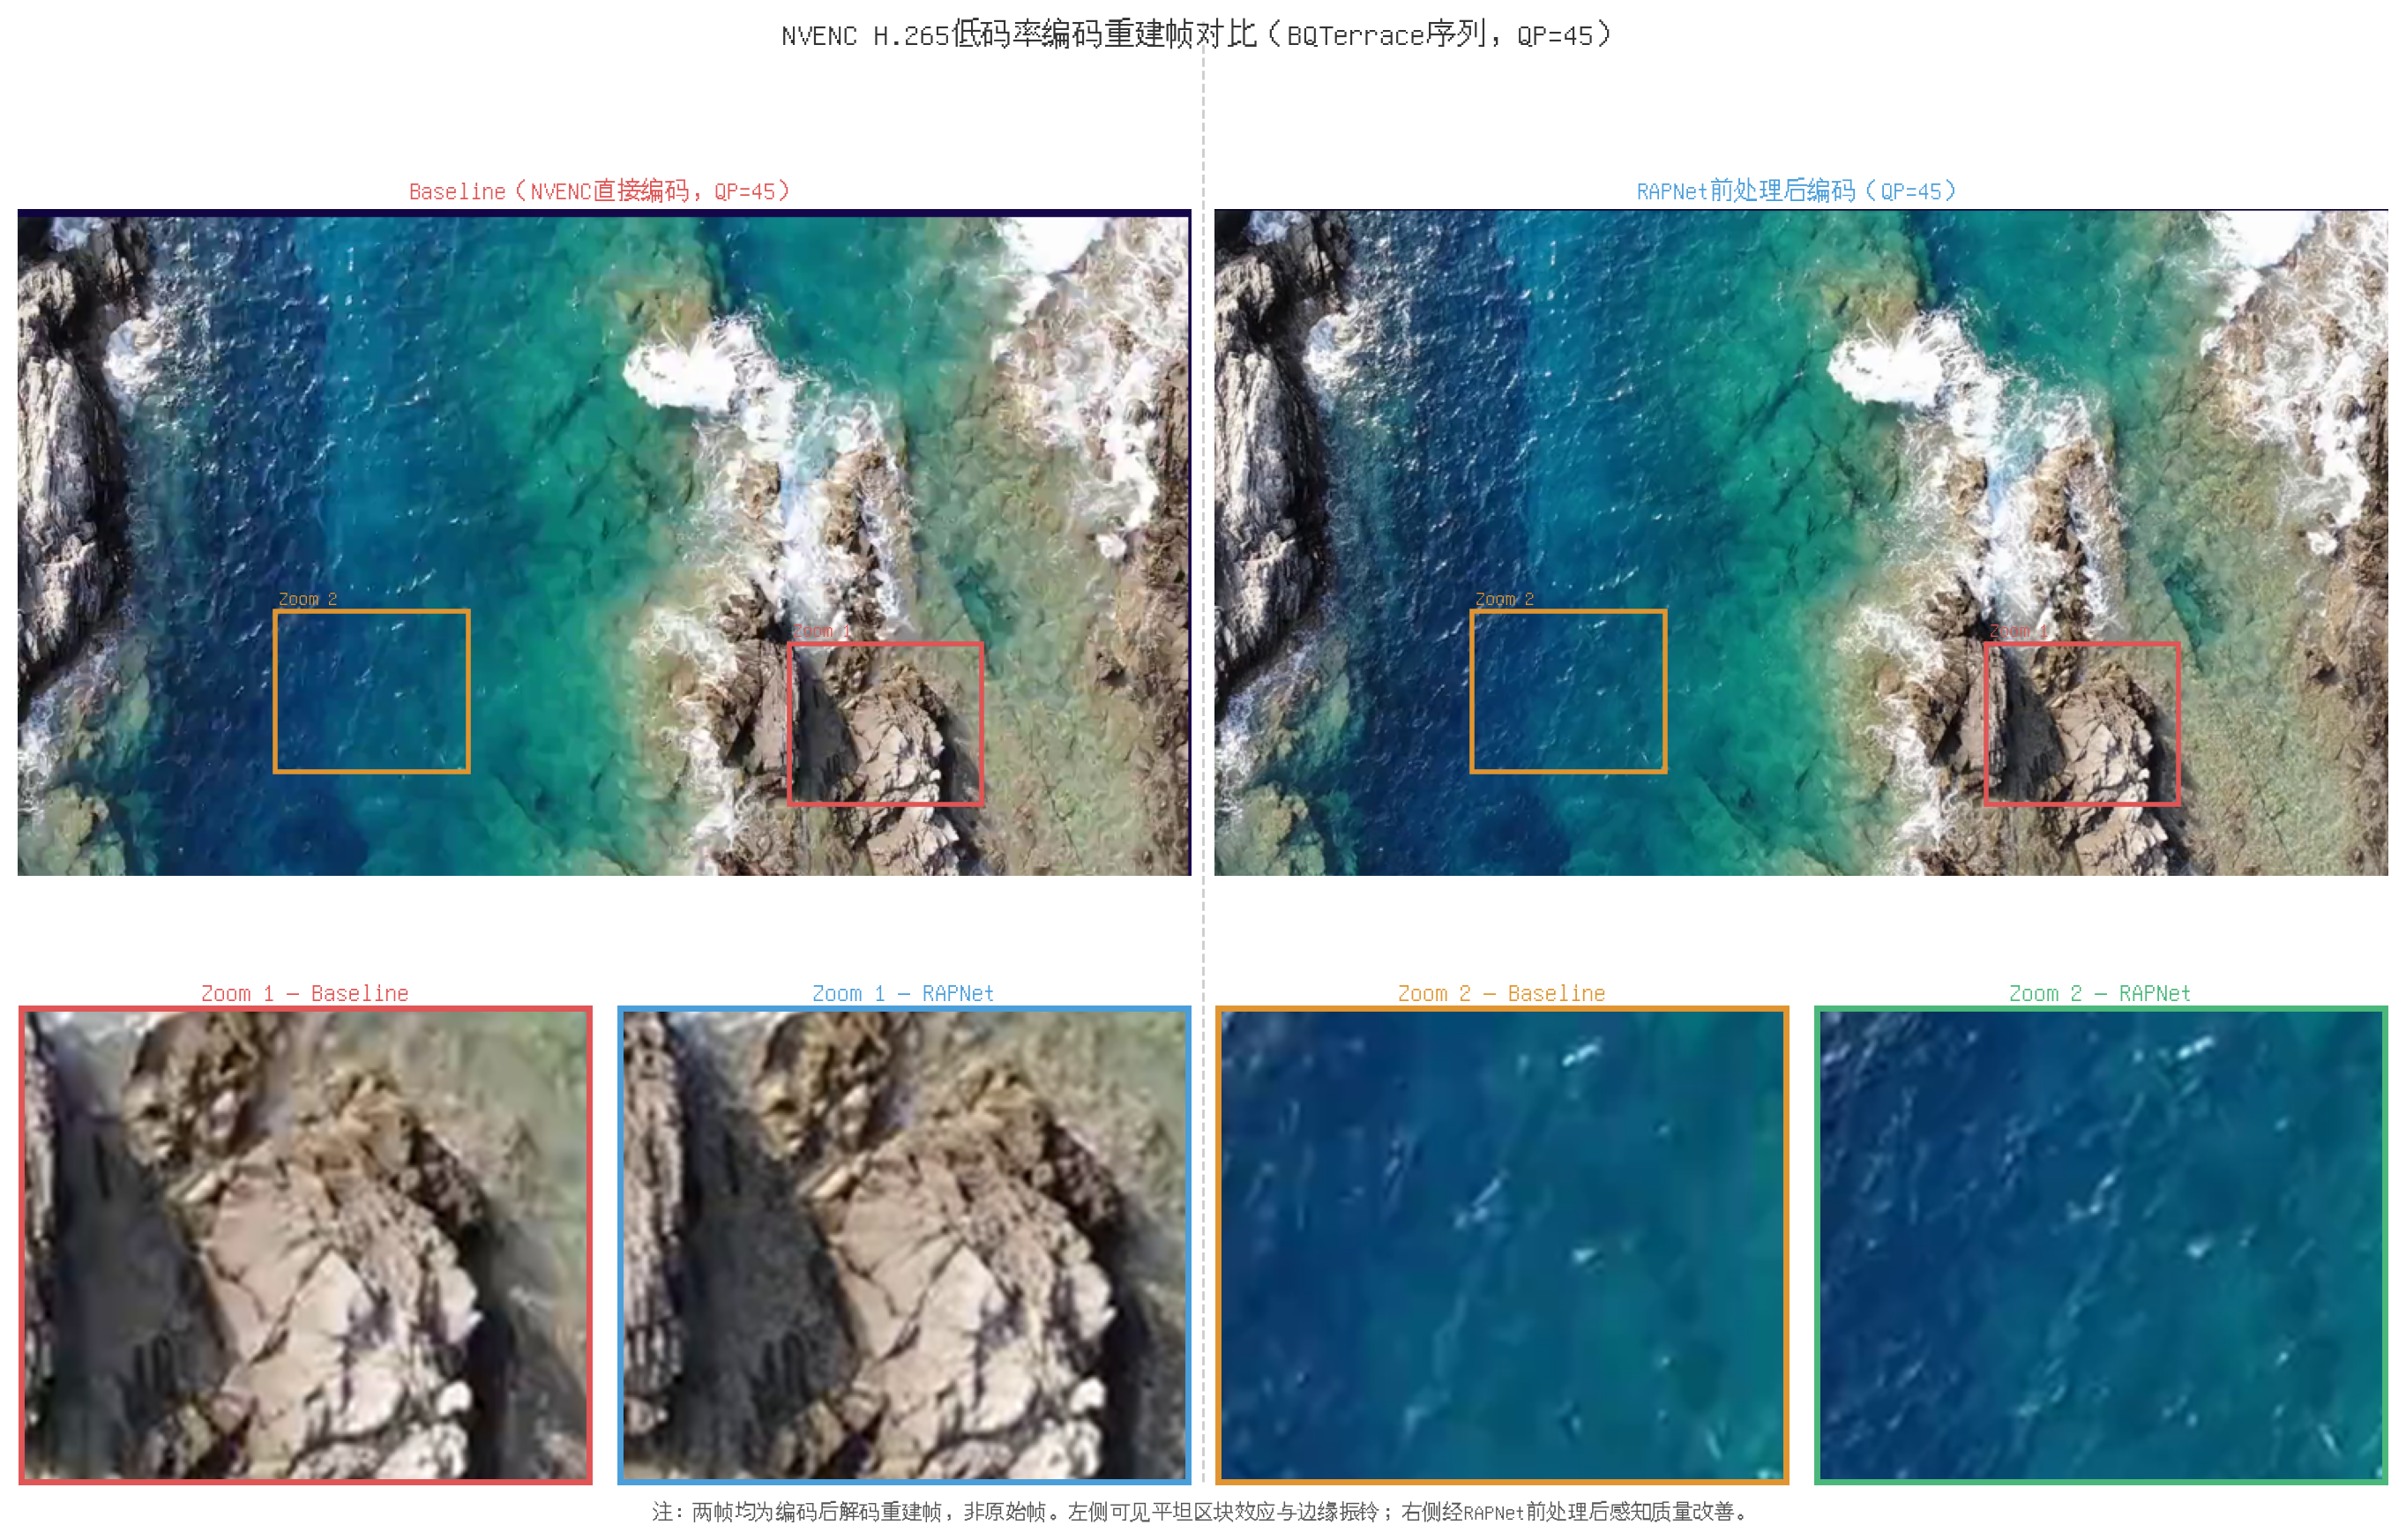
\includegraphics[width=\textwidth]{data/主观图片/background_blocking_comparison.png}
  \caption{NVENC H.265低码率编码重建帧对比（QP=45；两帧均为编码后解码重建帧）}
  \label{fig:background-blocking}
\end{figure}

针对低码率下的画质退化，已有研究提出了超分辨率、去噪和压缩伪影去除等深度增强模型，但这类模型直接用于实时编码仍存在困难。传统滤波方法可以减少部分高频噪声和码率开销，却容易造成过度平滑；基于Transformer的视频复原模型\cite{ref22-liang2022vrt,ref23-liang2022rvrt}虽然在公开数据集上表现较好，但参数量和推理耗时通常难以满足实时编码约束。陈彤等人在综述\cite{ref29-tong2025annual}中也指出，智能编码研究需要同时考虑率失真性能、计算复杂度、跨平台部署和低延迟要求。基于这一背景，本文将研究重点放在编码前处理环节，使模型在进入硬件编码器之前调整输入信号，而不是在解码后再进行离线修复。

相关的深度学习视频编码综述\cite{ref16-ding2021advances}明确指出，前处理的核心目标是在进入标准编码器之前，通过神经网络去除心理视觉冗余\footnote{心理视觉冗余（Psychovisual redundancy）是指人眼视觉系统(HVS)关注不到或不敏感的图像纹理和细节，将其滤除能在不影响主观感受的前提下大幅节省码率开销。}。这也是近年工业界优化编码管道的重要实践，正如bilibili团队\cite{ref17-ma2023rateperception}在RPP方案中所采取的策略：通过利用神经网络将对主观视觉影响较小、且编码开销极大的非本质高频信息\footnote{在视频编码语境中，此处的高频信息通常指人眼视觉系统不敏感的高频纹理或噪声干扰。适度滤除它们能够大幅减少残差能量，进而提升编码效率，同时基本不影响主观感受。}过滤为零，能够直接从源头减少残差能量，进而改善后续硬件编码器的熵编码效率。
    
基于上述问题，本文研究一种面向NVENC低码率视频编码的强化学习前处理方法。该方法不修改硬件编码器内部结构，而是在编码前引入强化学习前处理网络，将NVENC视为黑盒环境，并用真实编码反馈更新前处理策略。在本文实验设置下，系统以5个1080p测试序列为源数据，通过Random Crop构造$960\times540$编码clip；模型参数量为113K，平均前处理时延为5.4ms/帧，并取得平均$-9.48\%$的BD-LPIPS收益。

\section{国内外研究现状}

过去三十余年，主流视频编码技术路线始终围绕变换、预测、环路滤波等规则驱动的模块化工具展开精细化设计与协同优化，并依托MPEG、AVS、AOM等标准化组织构建起成熟的生态体系\cite{ref1-bross2021vvc}。尽管H.266/VVC等新一代标准的压缩效率持续提升，但在工业界大规模商用场景中，受限于极高的计算复杂度、编码时延以及复杂的专利布局，H.264/AVC与H.265/HEVC仍占据着绝对主导地位。

近十年来，随着深度神经网络的快速发展，视频编码领域迎来了新的变革\cite{ref16-ding2021advances}。当前研究已逐渐分化为两条路线：一条是全AI端到端架构，通过深度网络完全替代传统流程\cite{ref8-lu2019dvc,ref6-li2021deep,ref4-cong2025adaptive}，虽然在多个公开数据集上展现出优于H.265/HEVC的压缩效率\cite{ref10-sullivan2012hevc}，但其庞大的算力开销使其难以在边缘设备上部署；另一条是围绕固定硬件编码器进行前后处理协同的AI增强架构\cite{ref9-shen2011downsampling,ref11-vanam2023spie,ref12-vanam2023dcc}，在针对超分辨率\cite{ref2-chan2021basicvsr}、滤波去噪\cite{ref7-lin2019improved}、变换\cite{ref3-chen2018rl}、帧内帧间预测\cite{ref20-chen2023fastmfqe}等环节进行模块化替换或辅助增强。近期也有工作尝试将视频编解码器重新抽象为更通用的张量压缩基础设施\cite{ref18-xu2025llm265}，说明编码技术与AI系统之间的边界正在进一步模糊。后一条路线因其部署灵活、兼容H.26x标准的优势，成为当前工业界与学术界的研究热点。



\section{研究内容与主要工作}

本文提出了由硬件编码器、轻量前处理与AI后处理构成的视频编码增强框架。为突出研究对象与技术主线，本文聚焦于NVENC硬件编码链路中的前处理优化问题，重点研究前处理网络设计、强化学习训练机制及其对率失真性能的影响；后处理联合优化仅作为整体系统背景，不在本文中重点展开。基于上述范围界定，本文的主要工作包括：

\begin{enumerate}
  \item \textbf{课题研究与方案设计}：调研分析H.265硬件编码(NVENC)相较于软件编码的优劣势，特别是其在低功耗、高效率方面的特点以及可能存在的率失真性能损失问题。研究硬件编码结合轻量前处理的视频编码落地路径，设计一套兼顾低功耗和率失真性能的混合编码框架；
  \item \textbf{系统实现与模型构建}：搭建实验系统，集成NVENC硬件编码器，实现基于强化学习的RAPNet\cite{ref27-zhao2025rapnet}前处理算法，AI算法的模型参数量控制在1M以内；
  \item \textbf{实验验证与性能评估}：使用HEVC CTC Class B中的1080p分辨率、YUV420格式标准测试序列\cite{ref-bossen2013ctc}作为源数据，在训练与评测阶段随机裁剪$960\times540$区域构造编码clip，并在CQP模式下以QP$\in\{37,40,42,45,47\}$五个测试点进行量化验证，对比BD-LPIPS感知率失真收益、主观视觉效果、计算复杂度等指标。
\end{enumerate}

\section{本文创新点}

% 论文创新点

本文的主要创新点如下：

\begin{enumerate}
  \item \textbf{编码器感知的强化学习前处理框架}。针对NVENC等硬件编码器"不可导"的固有限制，本文提出将其作为强化学习中的"黑盒环境"纳入优化回路。通过Actor-Critic架构，系统以NVENC编码后的实际码率和感知质量（LPIPS）作为奖励信号，使前处理网络RAPNet能够在不依赖编码器梯度的前提下，自适应地学习针对硬件编码器特性的预补偿策略，有效缓解了低码率场景下的质量崩塌问题。

  \item \textbf{基于Random Crop的高频保持训练策略}。区别于传统的下采样训练方式（如2$\times$下采样到540p），本文采用从1080p原始帧中随机裁剪540$\times$960区域的训练策略。该策略在保持与下采样方案相同计算开销的前提下，完整保留了原始视频的高频纹理和边缘细节，避免了下采样导致的信息丢失，使模型能够学习到更精细的增强策略。

  \item \textbf{频域感知的复合损失函数设计}。除策略梯度损失外，本文设计了一套基于空间频率分解的辅助损失体系：（1）低频结构保持损失（通过$5 \times 5$均值滤波约束低频内容一致性）；（2）非边缘区域高频抑制损失（利用Sobel边缘检测生成软掩模，仅在平坦区域惩罚高频修改，避免边缘模糊）；（3）边缘聚焦损失（鼓励模型将修改集中在边缘区域，提升主观锐度）。该设计使模型在提升编码效率的同时保持了视觉自然度。
\end{enumerate}

\section{论文结构安排}

本文共分为五章，各章内容安排如下：

第一章为绪论，介绍研究背景与意义、国内外研究现状概述、研究内容与主要工作、本文创新点以及论文结构安排。

第二章为相关工作与理论基础，系统梳理视频编码标准演进、编码器感知前处理技术发展脉络、后处理技术分析以及强化学习基础理论，并结合模型复杂度与性能分析，明确本文的技术选型依据。

第三章详细阐述系统设计与实现，包括基于Actor-Critic架构的视频前处理优化系统的整体设计、状态空间与动作空间的定义、复合奖励函数设计及网络损失函数建模。

第四章进行实验与结果分析，在多个QP测试点上对比基线编码与集成增强前处理，从BD-LPIPS、主观视觉效果、计算复杂度等维度验证方案；同时分析近50个强化学习训练版本，总结通道崩塌、梯度爆炸等失败案例及工程处理方法。

第五章总结全文，分析方案局限，并展望端到端联合优化等后续工作。
  % 第一章：绪论
\chapter{国内外研究现状与理论基础}

\section{视频编码标准演进}

视频编码标准的发展经历了多个重要里程碑。从早期的H.261到如今的H.266/VVC，每一代标准都在压缩效率上取得了显著提升\cite{ref19-badawy2025evolution}。本节简要回顾视频编码标准的发展脉络及其核心技术特点。

\subsection{H.265/HEVC标准}

H.265/HEVC (High Efficiency Video Coding) 由ITU-T VCEG和ISO/IEC MPEG联合开发，于2013年正式发布\cite{ref10-sullivan2012hevc}。相比H.264/AVC，HEVC在同等主观质量下可节省约50\%的码率。其核心技术改进包括：

\begin{itemize}
  \item 灵活的编码树单元(CTU)划分结构，最大支持$64 \times 64$像素块；
  \item 增强的帧内预测模式，支持35种角度预测方向；
  \item 改进的环路滤波器，包括去块效应滤波器(DBF)和样本自适应偏移(SAO)滤波器。
\end{itemize}

\subsection{H.266/VVC标准}

H.266/VVC (Versatile Video Coding)于2020年发布，在HEVC的基础上进一步提升了约30\%--50\%的压缩效率\cite{ref1-bross2021vvc}。然而，其编码计算复杂度的激增使其在实时应用中面临巨大挑战。

\subsection{硬件编码器NVENC}

NVIDIA Video Encoder (NVENC) 是集成在NVIDIA GPU中的专用硬件编码引擎。与软件编码器(如x265)相比，NVENC具有以下特点：

\begin{itemize}
  \item 极低的编码延迟，支持实时1080p/4K编码；
  \item 低功耗，不占用CPU/GPU通用计算资源；
  \item 率失真性能可能不及软件编码器的最高质量模式。
\end{itemize}

% TODO: 可以在此补充NVENC与x265的性能对比数据

\section{前处理技术分析}

视频前处理的目标是在编码前优化原始信号，使其更适合压缩\cite{ref17-ma2023rateperception}。理想的模型需在计算复杂度、时域一致性与显存开销之间取得平衡。在低码率场景下，有效的降噪几乎等同于压缩。

\subsection{传统CNN架构}

以DnCNN\cite{ref5-ho2021rrdncnn}为代表的早期图像复原模型，结构简单但感受野有限，难以捕捉长距离依赖，容易导致过度平滑，丢失纹理细节。

\subsection{Transformer架构}

以SwinIR\cite{ref25-liang2021swinir}为代表的Transformer架构通过引入自注意力机制，能够有效建模全局依赖关系，在图像复原任务上取得了优异性能。然而，其计算复杂度随图像分辨率呈二次方增长，对于1080p及以上的高清视频处理，计算与显存开销巨大。值得注意的是，如VRT\cite{ref22-liang2022vrt}这类模型的惊人资源消耗是在仅为$320 \times 180$的低分辨率下测得的，若将其外推至1080p视频，其注意力机制的二次方复杂度将使其在任何实时应用中都变得完全不切实际。

% TODO: 可以插入表格对比各架构的参数量和推理耗时（参考开题报告中的表1、表2）

\subsection{状态空间模型架构}

以MambaIR\cite{ref21-guo2024mambaIRv2}为代表的新兴架构将计算复杂度降低至线性级别，同时保留了强大的长距离依赖建模能力。调研数据显示，MambaIR在去除噪声的同时，能比其他模型更好地保留边缘和纹理细节，有效避免了画面的过度"磨皮"效应，使其成为轻量级、高效视频前处理的理想选择。

\section{后处理技术分析}

后处理通常在解码后进行，旨在修复压缩过程中产生的失真（如块效应、振铃效应）并提升分辨率\cite{ref2-chan2021basicvsr}。主要代表性方法包括：

\begin{itemize}
  \item \textbf{VRT}\cite{ref22-liang2022vrt}：视频复原领域的性能标杆，全局注意力效果出众但推理极慢、显存占用极高；
  \item \textbf{RVRT}\cite{ref23-liang2022rvrt}：VRT的循环变体，显存占用约为VRT的一半，推理速度更快，是更具实用性的后处理方案；
  \item \textbf{BasicVSR++}\cite{ref2-chan2021basicvsr,ref24-wang2022basicsr}：经典循环网络模型，以极低参数量和极快推理速度成为视频增强领域的高效基准。
\end{itemize}

% TODO: 可以插入表格对比各模型的复杂度与性能（参考开题报告中的表3、表4）

\section{强化学习基础}

\subsection{马尔可夫决策过程}

强化学习问题通常建模为马尔可夫决策过程(MDP)，由五元组 $(S, A, P, R, \gamma)$ 描述：

\begin{itemize}
  \item $S$：状态空间；
  \item $A$：动作空间；
  \item $P$：状态转移概率；
  \item $R$：奖励函数；
  \item $\gamma$：折扣因子。
\end{itemize}

\subsection{Actor-Critic架构}

Actor-Critic是一种结合了策略梯度方法(Actor)和价值估计方法(Critic)的混合架构\cite{ref26-liu2021elegantrl}。Actor负责根据当前状态选择动作，Critic负责评估当前状态-动作对的价值。其优势在于：

\begin{enumerate}
  \item 通过Critic的价值估计降低策略梯度的方差；
  \item Actor可以输出连续动作，适用于图像增强等高维连续空间任务。
\end{enumerate}

在视频编码领域，文献\cite{ref3-chen2018rl}已证明强化学习能有效应用于HEVC帧级码率分配；AVS M9322提案\cite{ref27-zhao2025rapnet}进一步将其扩展到基于RAPNet的前处理滤波工具中，证明了强化学习在提升编码器率失真性能方面的巨大潜力。

\section{本章小结}

本章首先回顾了视频编码标准的演进历程，重点分析了H.265/HEVC标准\cite{ref10-sullivan2012hevc}及NVENC硬件编码器的特点。随后对主流的前处理与后处理技术进行了分类分析，涵盖了CNN\cite{ref5-ho2021rrdncnn}、Transformer\cite{ref25-liang2021swinir,ref22-liang2022vrt}和状态空间模型\cite{ref21-guo2024mambaIRv2}三类架构的优缺点。最后介绍了强化学习中马尔可夫决策过程和Actor-Critic架构的基本理论，为后续章节的系统设计提供了理论基础。
  % 第二章：国内外研究现状与理论基础
\chapter{系统设计与实现}

本章详细阐述基于Actor-Critic架构的视频前处理优化系统的整体设计与实现。系统的核心思想是将不可导的硬件编码器(NVENC)纳入到强化学习的优化回路中，通过"编码器感知"的方式使前处理模型能够针对硬件编码器的特性（如量化步长、块划分模式）\cite{ref6-li2021deep}进行预补偿，有效缓解低码率场景下的质量崩塌。

% ============================================================
% 【示例：如何插入图片】
% 将图片文件放入项目根目录的 data/ 文件夹中
% ============================================================
% \begin{figure}[htbp]
%   \centering
%   \includegraphics[width=0.85\textwidth]{data/system_overview.png}
%   \caption{基于Actor-Critic架构的视频前处理优化系统框图}
%   \label{fig:system-overview}
% \end{figure}

\section{系统总体架构}

本文提出的协处理系统整体框架如图~\ref{fig:pipeline}所示，主要由三个部分组成：

\begin{enumerate}
  \item \textbf{轻量级AI前处理模块}(RAPNet)\cite{ref27-zhao2025rapnet}：采用基于强化学习的码率自适应前处理网络，在编码前对原始视频帧进行智能增强；
  \item \textbf{硬件编码器}(NVENC)：利用NVIDIA GPU中的专用编码引擎对增强后的视频进行H.265编码\cite{ref10-sullivan2012hevc}；
  \item \textbf{AI后处理模块}：在解码端对重建视频进行质量增强与超分辨率处理\cite{ref2-chan2021basicvsr}。
\end{enumerate}

% TODO: 替换为系统总体架构图
\begin{figure}[htbp]
  \centering
  % \includegraphics[width=0.9\textwidth]{data/pipeline.png}
  \fbox{\parbox{0.8\textwidth}{\centering\vspace{3cm}请替换为系统总体架构图\\（将图片放到 data/ 文件夹后取消上方注释）\vspace{3cm}}}
  \caption{前后处理整体流程}
  \label{fig:pipeline}
\end{figure}


\section{状态空间与动作空间设计}

\subsection{状态空间构建}

定义$t$时刻的状态空间$s_t$为待编码的原始视频帧序列。鉴于NVENC硬件编码器及主流视频标准广泛采用YCbCr 4:2:0格式，系统首先通过双线性插值(Bilinear Interpolation)将下采样的色度分量(Cb, Cr)上采样至与亮度分量(Y)相同的空间分辨率。最终构建的输入状态张量形状为$(B \times T, 3, H, W)$，其中$T$为时序长度，旨在利用视频帧间的时域相关性辅助决策。

\subsection{动作空间定义}

为了克服直接生成像素可能导致的训练震荡与收敛困难问题，系统采用\textbf{残差学习}(Residual Learning)策略。Agent的输出并非直接的像素值，而是针对原始帧的残差修正量。定义$t$时刻的状态为原始视频帧$s_t$，网络输出为残差图$f_{\text{Actor}}(s_t)$，则最终生成的动作$a_t$表示为：

% ============================================================
% 【示例：如何插入公式】
% ============================================================
\begin{equation}
  a_t = \text{clamp}(s_t + f_{\text{Actor}}(s_t), 0, 1)
  \label{eq:action}
\end{equation}

其中，$\text{clamp}(\cdot, 0, 1)$ 操作用于将叠加后的像素值强制约束在合法区间 $[0, 1]$ 内，确保输入硬件编码器的视频帧数据有效。


\section{复合奖励函数设计}

针对低码率场景下"主观画质"与"传输带宽"的博弈难题，设计了基于参考率失真(Reference Rate-Distortion)特性的复合奖励函数。该函数旨在引导模型在相对于基准编码器(Baseline)的相对增益中寻找平衡点，其数学形式定义如下：

\begin{equation}
  R_{total} = \alpha \cdot \frac{Q_{act} - Q_{ref}}{Q_{ref}} - \beta \cdot \frac{R_{act} - R_{ref}}{R_{ref}}
  \label{eq:reward}
\end{equation}

式中，$Q_{act}$ 和 $R_{act}$ 分别为当前动作经NVENC编码后解码获得的感知质量分数（采用LPIPS取负）和实际码率；$Q_{ref}$ 和 $R_{ref}$ 为基准编码器在同等量化参数(QP)下的参考值。$\alpha$ 与 $\beta$ 为超参数，分别用于调控感知质量增益与码率惩罚的权重。


\section{网络损失函数建模}

为了确保Actor-Critic架构的稳定收敛，针对Critic和Actor网络分别设计了差异化的优化目标。

\subsection{Critic网络损失}

Critic网络(ValueNet)旨在准确评估当前策略的价值，其训练目标是最小化预测$Q$值与真实奖励$R_{total}$之间的均方误差(MSE)：

\begin{equation}
  \mathcal{L}_{\text{Critic}} = \text{MSE}(V(s_t, a_t), R_{total})
  \label{eq:critic-loss}
\end{equation}

\subsection{Actor网络损失}

Actor网络(RAPNet)的损失函数采用复合损失策略，由策略梯度损失、像素级内容一致性损失(Pixel Loss)以及全变分平滑损失(Total Variation Loss)三部分加权构成：

\begin{equation}
  \mathcal{L}_{\text{Actor}} = \mathcal{L}_{\text{policy}} + \lambda \cdot \mathcal{L}_{\text{pixel}} + \mu \cdot \mathcal{L}_{\text{TV}}
  \label{eq:actor-loss}
\end{equation}

各项的具体定义如下：

\textbf{（1）策略梯度损失}$\mathcal{L}_{\text{policy}}$：旨在最大化Critic对当前动作的评分，引导网络生成高回报的增强帧：
\begin{equation}
  \mathcal{L}_{\text{policy}} = -\mathbb{E}[V(s_t, f_{\text{Actor}}(s_t))]
  \label{eq:policy-loss}
\end{equation}

\textbf{（2）像素级一致性损失}$\mathcal{L}_{\text{pixel}}$：用于约束生成帧与原始帧在低频内容上的结构一致性，防止色彩偏移。采用加权均方误差形式（亮度通道权重更高）：
\begin{equation}
  \mathcal{L}_{\text{pixel}} = 6 \cdot \text{MSE}(Y, \hat{Y}) + 1 \cdot \text{MSE}(C_b, \hat{C}_b) + 1 \cdot \text{MSE}(C_r, \hat{C}_r)
  \label{eq:pixel-loss}
\end{equation}

\textbf{（3）全变分平滑损失}$\mathcal{L}_{\text{TV}}$：为了抑制由卷积操作引起的棋盘格伪影及高频噪声，引入各向异性全变分损失(Anisotropic Total Variation Loss)。该损失通过最小化相邻像素间的差异来提升图像的空间平滑度：
\begin{equation}
  \mathcal{L}_{\text{TV}} = \frac{1}{N} \sum_{b,c,h,w} \left[ (\hat{x}_{b,c,h+1,w} - \hat{x}_{b,c,h,w})^2 + (\hat{x}_{b,c,h,w+1} - \hat{x}_{b,c,h,w})^2 \right]
  \label{eq:tv-loss}
\end{equation}

其中，$N = B \times C \times H \times W$ 为归一化因子，确保损失数值不随分辨率变化而波动；$\hat{x}$ 代表Actor输出的增强帧。

\section{RAPNet网络架构}

RAPNet (Rate-Adaptive Pre-processing Network)\cite{ref27-zhao2025rapnet} 采用具备线性复杂度的轻量级架构，参数量严格控制在1M以内。本项目摒弃了计算开销巨大的Transformer架构\cite{ref22-liang2022vrt}，创新性地选用了具备线性复杂度的轻量级网络作为核心骨干\cite{ref17-ma2023rateperception}。其核心设计思想包括：

\begin{itemize}
  \item 采用残差学习策略，输出残差修正量而非直接像素值；
  \item 利用线性状态空间建模捕获长距离依赖关系\cite{ref21-guo2024mambaIRv2}；
  \item 支持1080p高清视频的实时推理，确保在端侧设备中的落地可行性。
\end{itemize}

% TODO: 插入RAPNet的网络结构图
% \begin{figure}[htbp]
%   \centering
%   \includegraphics[width=0.75\textwidth]{data/rapnet_arch.png}
%   \caption{RAPNet网络结构}
%   \label{fig:rapnet-arch}
% \end{figure}


\section{编码环境搭建}

系统基于NVIDIA Codec SDK搭建真实编码环境，通过Python的\texttt{subprocess}模块实现视频帧在Tensor与硬件编码器之间的实时交互。整体技术路线遵循"感知-决策-反馈-优化"的闭环路径：前处理后的视频输入硬件编码器生成比特流，系统计算重建帧与原始帧之间的感知损失(LPIPS)并获取实际码率，将此反馈计算奖励信号回传。在具体的模型迭代中，通过多轮离线预训练与特定场景UVG数据集\cite{ref28-mercat2020uvg}的在线微调，提升模型在复杂动态背景下的稳定性。

% ============================================================
% 【示例：如何插入代码】
% ============================================================
\begin{lstlisting}[language=Python, caption={NVENC编码调用示例}, label={lst:nvenc-call}]
import subprocess

def encode_with_nvenc(input_yuv, output_h265, width, height, qp):
    """使用NVENC硬件编码器进行H.265编码"""
    cmd = [
        'ffmpeg', '-y',
        '-f', 'rawvideo',
        '-pix_fmt', 'yuv420p',
        '-s', f'{width}x{height}',
        '-i', input_yuv,
        '-c:v', 'hevc_nvenc',
        '-qp', str(qp),
        output_h265
    ]
    subprocess.run(cmd, check=True)
\end{lstlisting}


\section{本章小结}

本章详细阐述了基于Actor-Critic架构的视频前处理优化系统的设计与实现。首先介绍了系统的总体架构，然后定义了状态空间与动作空间，设计了基于相对率失真增益的复合奖励函数，并建模了Critic和Actor网络的损失函数。最后介绍了RAPNet的网络架构和编码环境的搭建方式。  % 第三章：系统设计与实现
\chapter{实验与结果分析}

\section{实验环境与配置}

\subsection{硬件环境}

% ============================================================
% 【示例：三线表（使用 booktabs 宏包）】
% ============================================================
\begin{table}[htbp]
  \centering
  \caption{实验硬件环境配置}
  \label{tab:hardware}
  \begin{tabular}{ll}
    \toprule
    \textbf{配置项} & \textbf{参数} \\
    \midrule
    CPU         & Intel Core i9-13900K \\  % TODO: 改成你实际的配置
    GPU         & NVIDIA RTX 4090 (24GB) \\
    内存        & 64 GB DDR5 \\
    操作系统    & Ubuntu 22.04 LTS \\
    \bottomrule
  \end{tabular}
\end{table}

\subsection{软件环境}

\begin{table}[htbp]
  \centering
  \caption{实验软件环境配置}
  \label{tab:software}
  \begin{tabular}{ll}
    \toprule
    \textbf{软件/库} & \textbf{版本} \\
    \midrule
    Python       & 3.10 \\  % TODO: 改成你实际的版本
    PyTorch      & 2.1.0 \\
    CUDA         & 12.1 \\
    FFmpeg       & 6.0 \\
    NVIDIA Video Codec SDK & 12.0 \\
    ElegantRL\cite{ref26-liu2021elegantrl} & -- \\
    \bottomrule
  \end{tabular}
\end{table}

\subsection{数据集}

实验使用UVG数据集\cite{ref28-mercat2020uvg}中的1080p分辨率、YUV420格式（NV12转换）视频序列进行测试，序列时长至少为3秒。

\begin{table}[htbp]
  \centering
  \caption{测试视频序列}
  \label{tab:sequences}
  \begin{tabular}{lccl}
    \toprule
    \textbf{序列名称} & \textbf{分辨率} & \textbf{帧率} & \textbf{内容描述} \\
    \midrule
    BasketballDrive  & $1920 \times 1080$ & 50fps  & 运动场景（篮球） \\
    ParkScene        & $1920 \times 1080$ & 24fps  & 自然风景（公园） \\
    Kimono1          & $1920 \times 1080$ & 24fps  & 人物动作（和服） \\
    Cactus           & $1920 \times 1080$ & 50fps  & 复杂纹理（仙人掌） \\
    BQTerrace        & $1920 \times 1080$ & 60fps  & 城市场景（广场） \\
    \bottomrule
  \end{tabular}
\end{table}


\section{评价指标}

本文采用以下指标对实验结果进行评价：

\begin{itemize}
  \item \textbf{BD-Rate (Bjøntegaard Delta Rate)}：衡量两条率失真曲线之间码率节省百分比，负值表示节省码率；
  \item \textbf{LPIPS (Learned Perceptual Image Patch Similarity)}：基于深度学习的感知质量评价指标，值越低越好；
  \item \textbf{SSIM (Structural Similarity Index)}：结构相似性指标，范围$[0, 1]$，越高越好；
  \item \textbf{PSNR (Peak Signal-to-Noise Ratio)}：峰值信噪比，单位dB，越高越好；
  \item \textbf{模型参数量}：衡量模型复杂度，单位为K/M参数个数；
  \item \textbf{推理时间}：单帧推理耗时，衡量实时性。
\end{itemize}


\subsection{BD-LPIPS分析}

实验结果表明，基于强化学习的RAPNet前处理框架在LPIPS感知质量指标上相比Baseline取得了显著的BD-LPIPS优化。各视频序列的详细测试结果如表~\ref{tab:bdlpips-results}所示。

\begin{table}[htbp]
  \centering
  \caption{RAPNet前处理框架测试结果}
  \label{tab:bdlpips-results}
  \begin{tabular}{lcccc}
    \toprule
    \textbf{视频序列} & \textbf{Baseline平均LPIPS} & \textbf{$\Delta$LPIPS(\%)} & \textbf{$\Delta$码率(\%)} & \textbf{BD-LPIPS(\%)} \\
    \midrule
    BasketballDrive  & 0.4664 & $-11.53$ & $+1.02$  & $\mathbf{-12.84}$ \\
    ParkScene        & 0.5313 & $-4.51$  & $-11.08$ & $\mathbf{-13.45}$ \\
    Kimono1          & 0.4513 & $-1.78$  & $+3.74$  & $\mathbf{-5.62}$  \\
    Cactus           & 0.4349 & $+1.92$  & $-13.62$ & $\mathbf{-11.15}$ \\
    BQTerrace        & 0.4250 & $+0.54$  & $-4.95$  & $\mathbf{-4.32}$  \\
    \midrule
    \textbf{平均(Average)} & \textbf{0.4618} & $\mathbf{-3.07}$ & $\mathbf{-4.98}$ & $\mathbf{-9.48}$ \\
    \bottomrule
  \end{tabular}
\end{table}

从表~\ref{tab:bdlpips-results}可以看出，RAPNet在所有测试序列上均取得了负的BD-LPIPS值，平均BD-LPIPS为$-9.48\%$，表明在相同感知质量下可节省约9.48\%的码率。其中，ParkScene和BasketballDrive序列的改善最为显著，BD-LPIPS分别达到$-13.45\%$和$-12.84\%$。值得注意的是，Cactus序列虽然LPIPS略有上升($+1.92\%$)，但码率大幅下降($-13.62\%$)，综合BD-LPIPS仍达到$-11.15\%$。

图~\ref{fig:rd-curve-results}展示了Baseline与RAPNet在所有测试序列上的平均RD曲线对比。可以看到，RAPNet的RD曲线在所有码率点上均低于Baseline，表明在相同码率下RAPNet能够提供更低的LPIPS（即更好的感知质量）。

\begin{figure}[htbp]
  \centering
  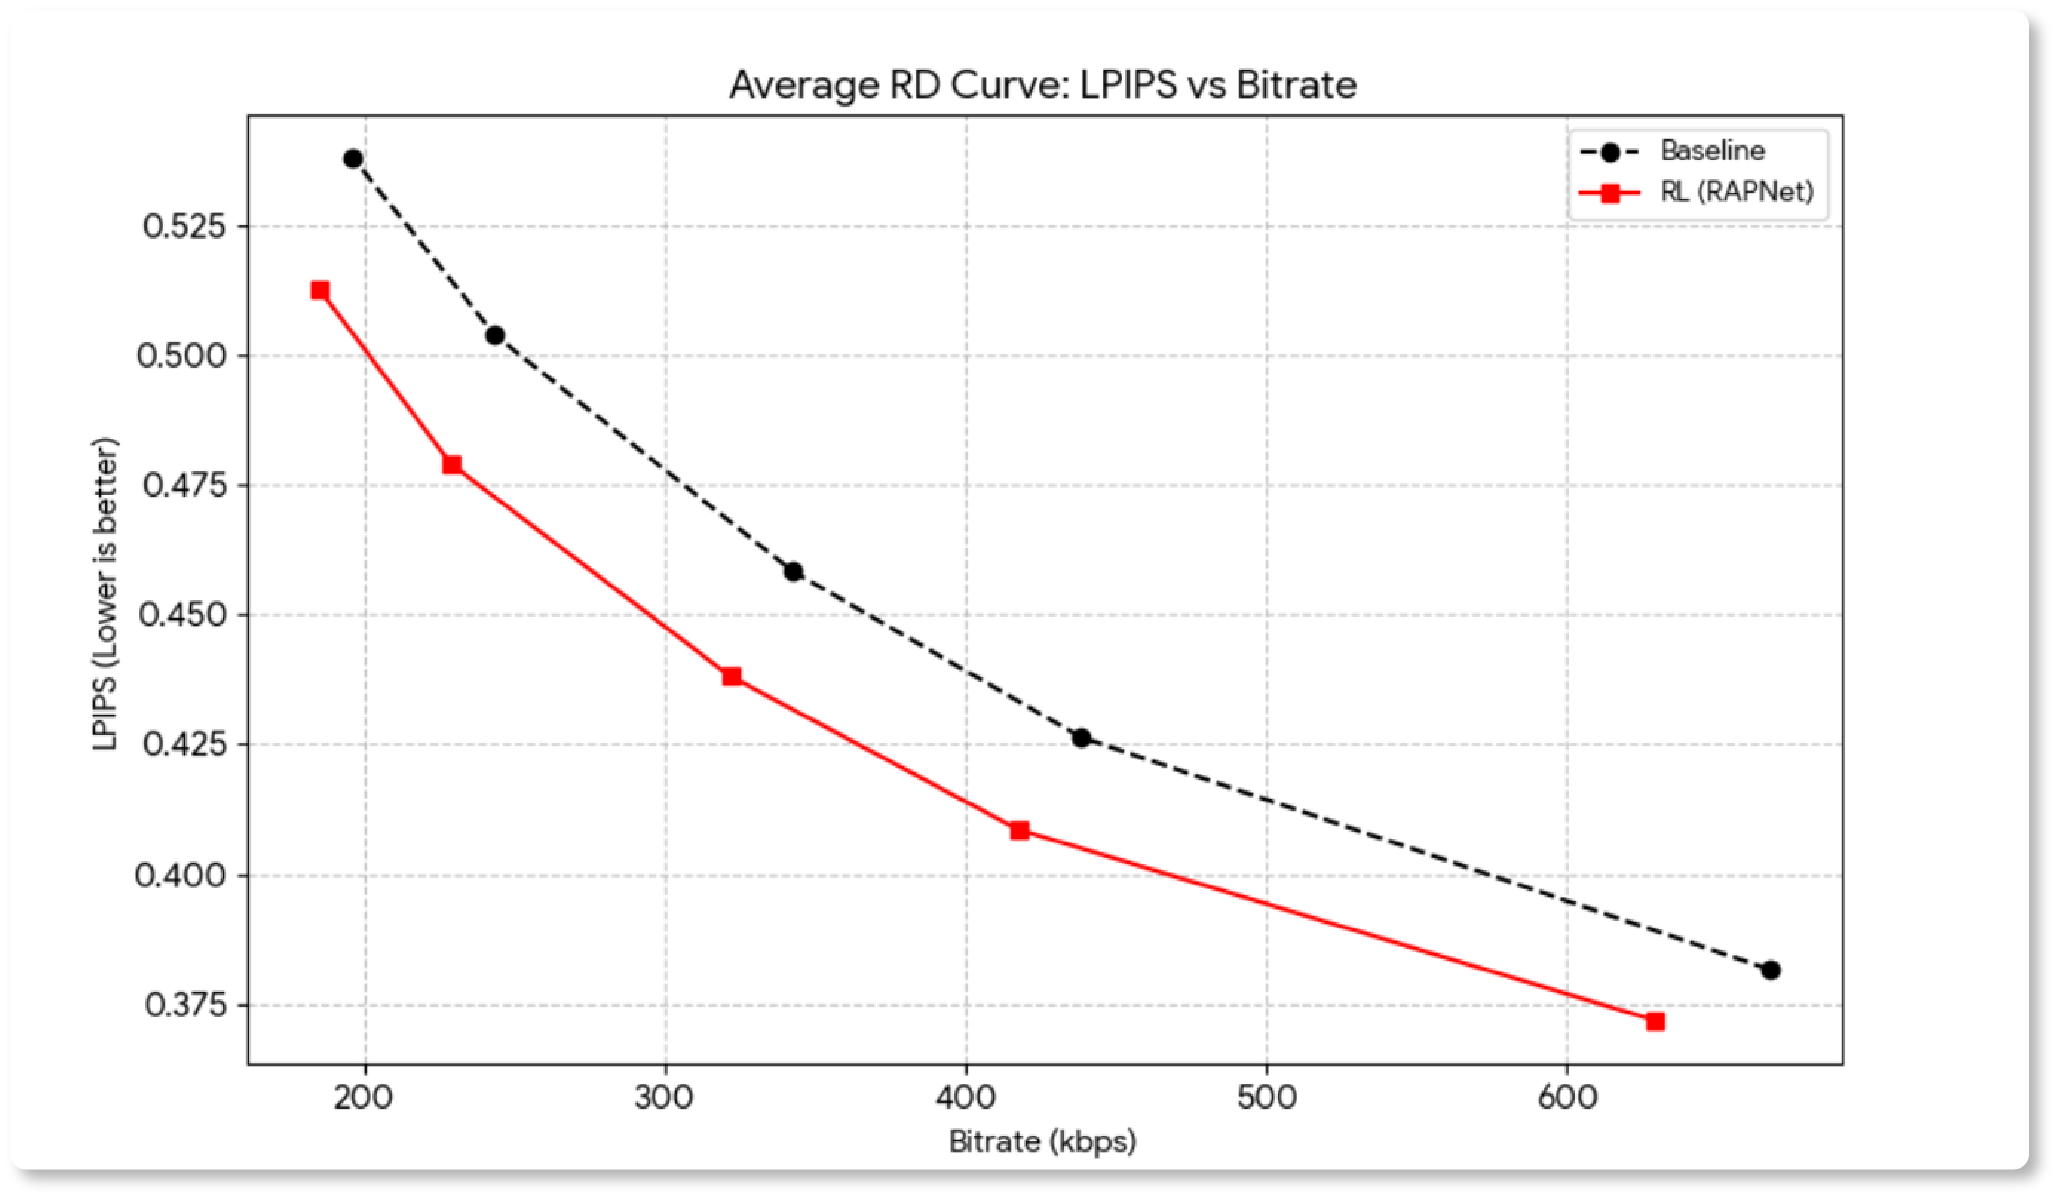
\includegraphics[width=0.75\textwidth]{data/图片测试结果RD曲线.png}
  \caption{Baseline与RAPNet平均RD曲线对比（LPIPS vs 码率）}
  \label{fig:rd-curve-results}
\end{figure}

\subsection{训练过程分析}

图~\ref{fig:training-curves}展示了训练过程中的关键监控指标。从TensorBoard训练曲线可以观察到：（1）delta\_r\_mean（码率节省）在训练前期波动较大，但整体呈正值趋势，表明模型学会了节省码率；（2）delta\_v\_mean（质量提升）在后半段训练中逐渐转正，表明感知质量得到改善；（3）force\_q\_thrust（Critic推力）和force\_mse\_drag（MSE阻力）的动态平衡反映了Actor-Critic架构中``探索与利用''的权衡过程。

\begin{figure}[htbp]
  \centering
  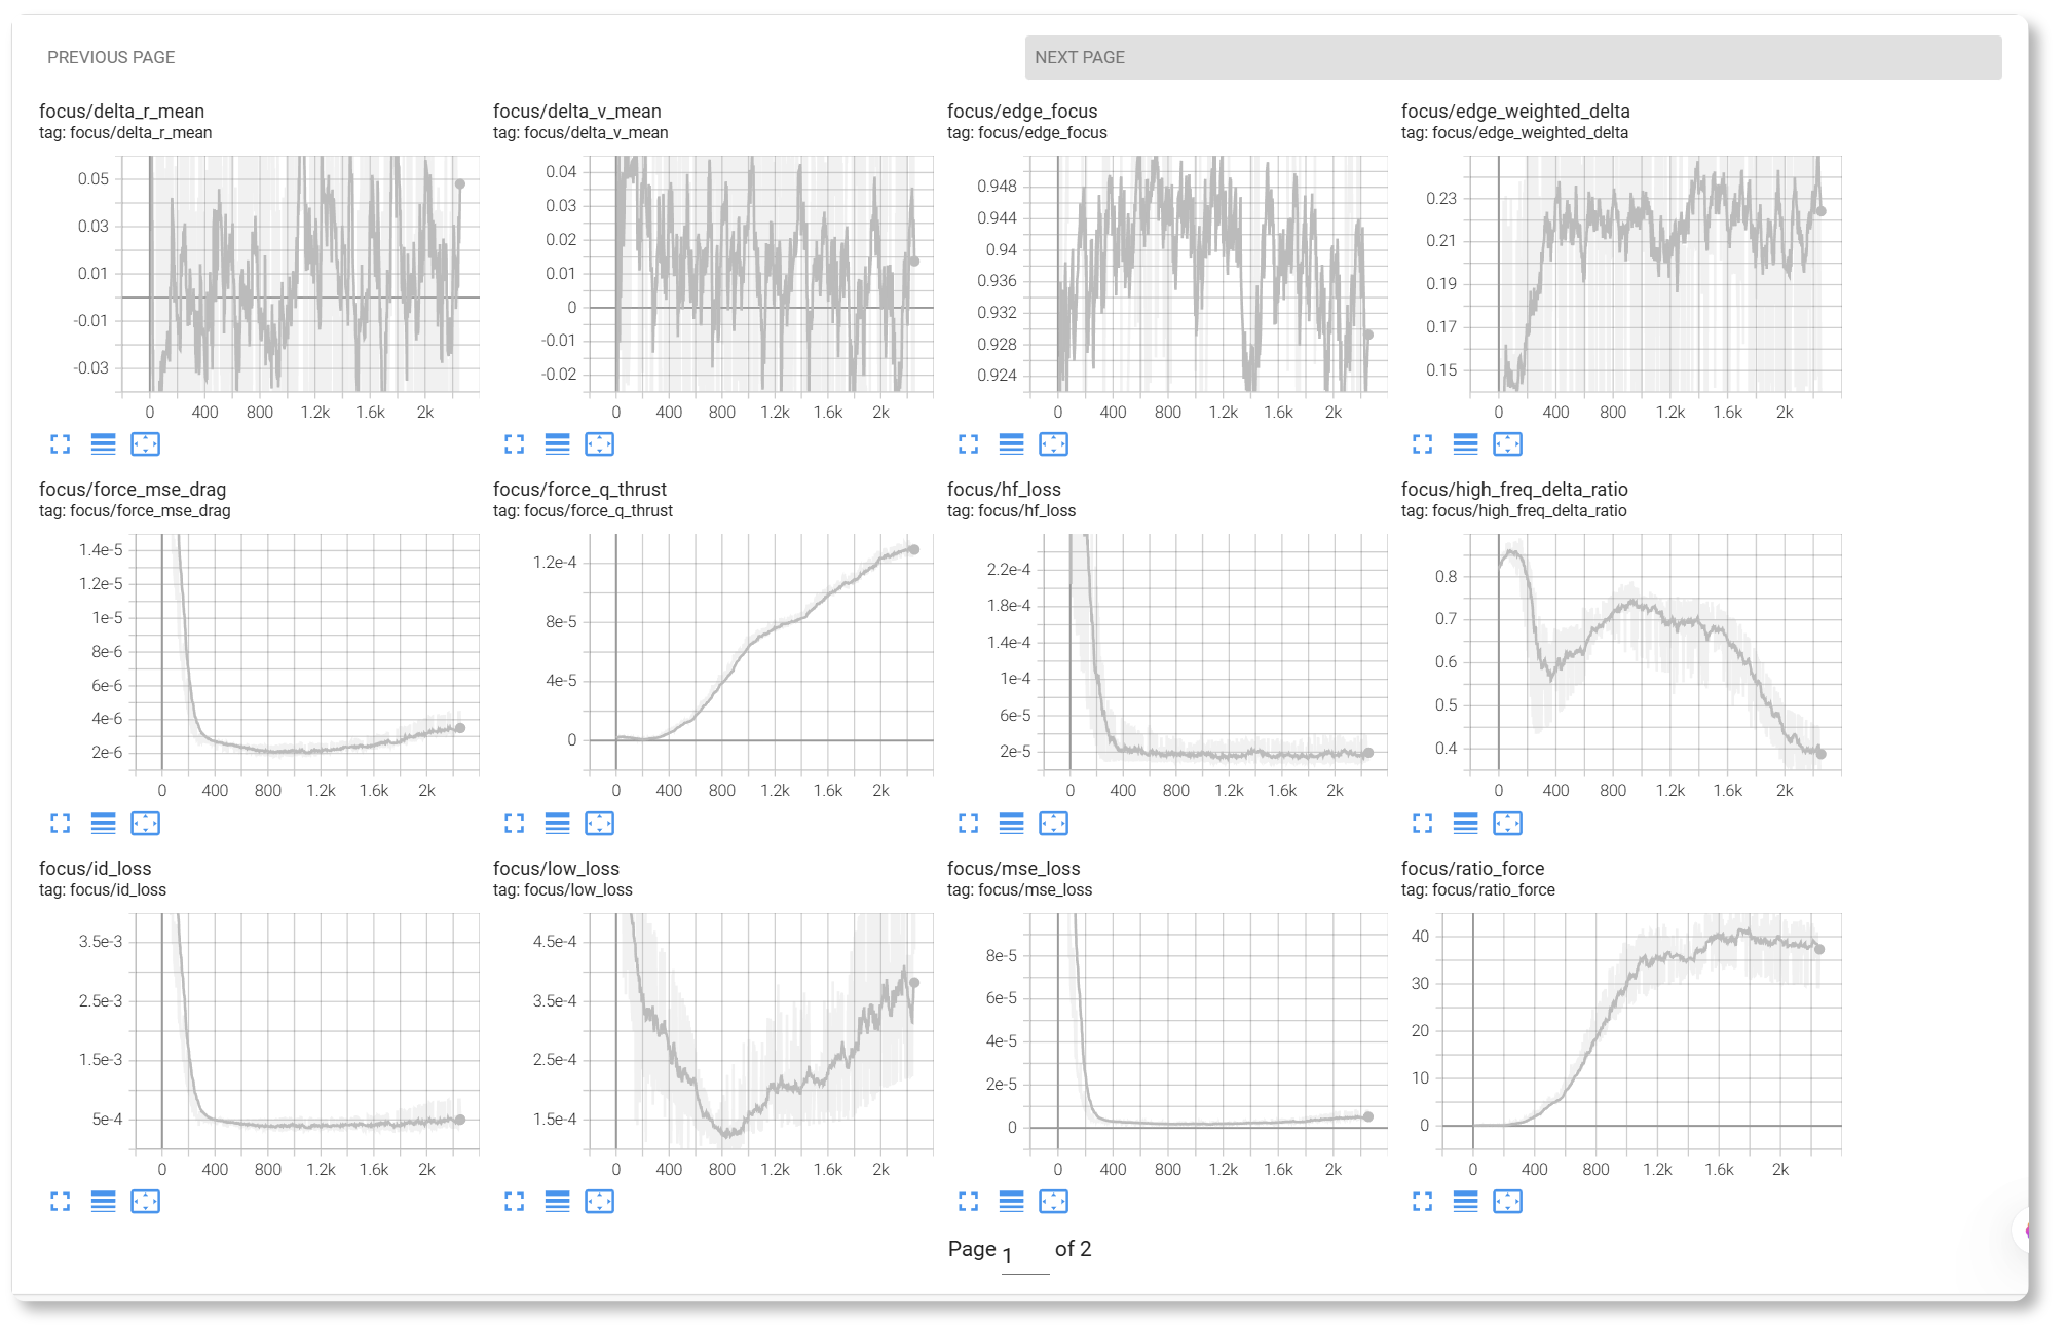
\includegraphics[width=0.95\textwidth]{data/图片训练曲线.png}
  \caption{TensorBoard训练监控曲线}
  \label{fig:training-curves}
\end{figure}

\subsection{频域分析}

图~\ref{fig:freq-training}展示了训练过程中图片频域的变化，可以观察到模型逐渐学会在特定频率方向上进行有针对性的修改。

\begin{figure}[htbp]
  \centering
  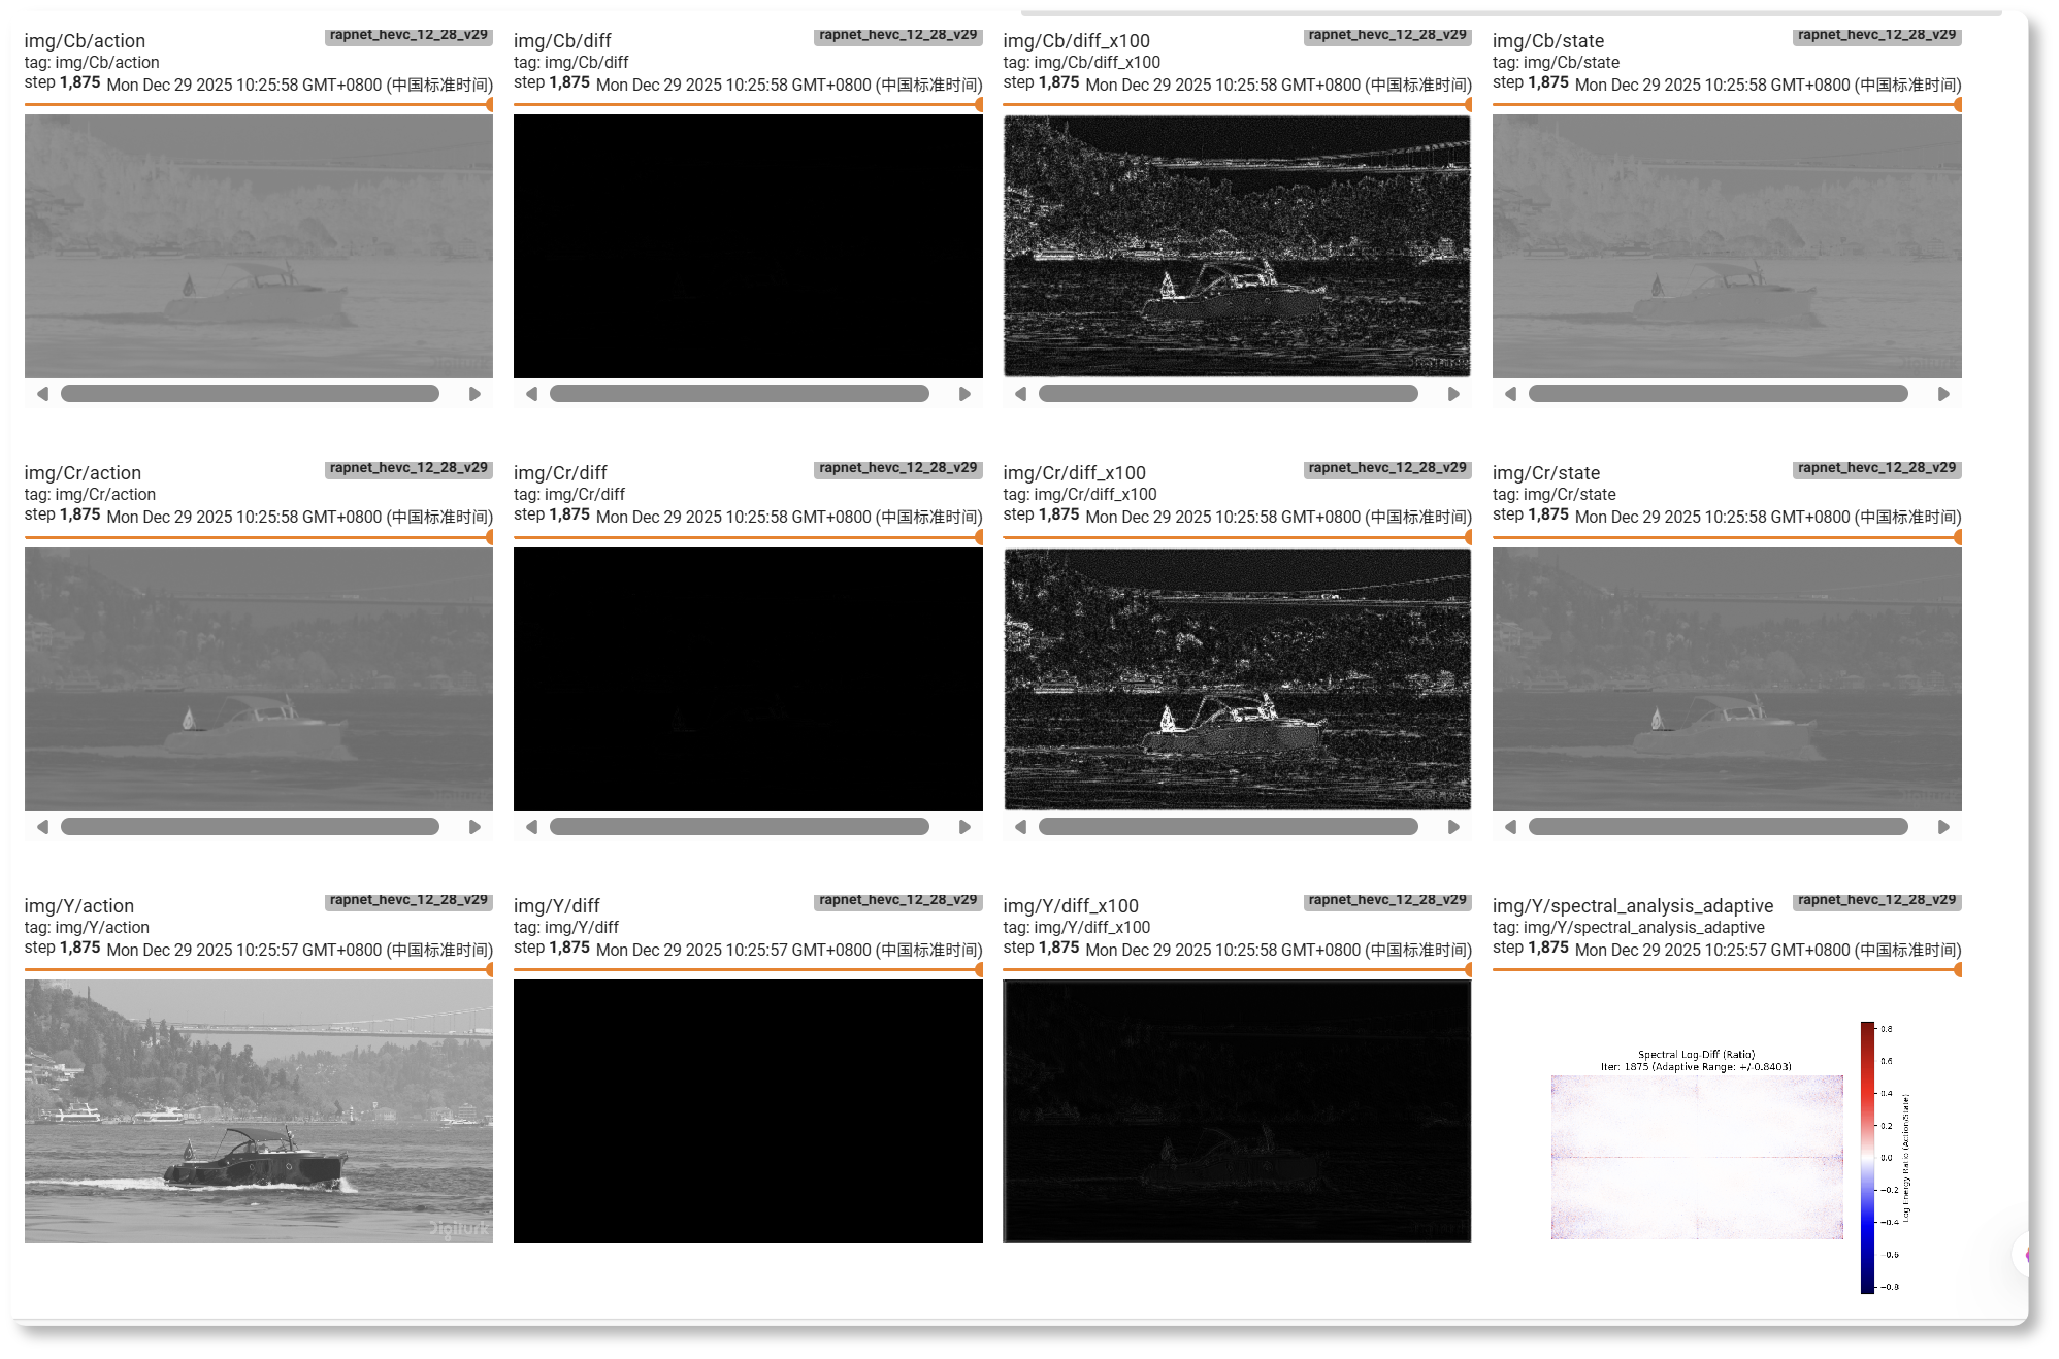
\includegraphics[width=0.95\textwidth]{data/图片训练过程中图片频域变化显示.png}
  \caption{训练过程中图片频域变化}
  \label{fig:freq-training}
\end{figure}

图~\ref{fig:spectrum-analysis}展示了经过充分训练后，模型处理前后图片的频谱差异图（Spectral Log-Diff）。可以看到图片经过模型处理后，主要有如下变化：频谱图在中心及四条边的中点位置出现有规律的红色增强，而四角区域几乎没有明显变化，说明网络主要保留了水平与垂直方向上的主结构分量，未显著增强斜向纹理。这种方向性增强更贴合自然图像的结构特征，同时也使得压缩后的内容在编码器的预测建模中更具可预测性，从而有助于整体编码效率的提升。

\begin{figure}[htbp]
  \centering
  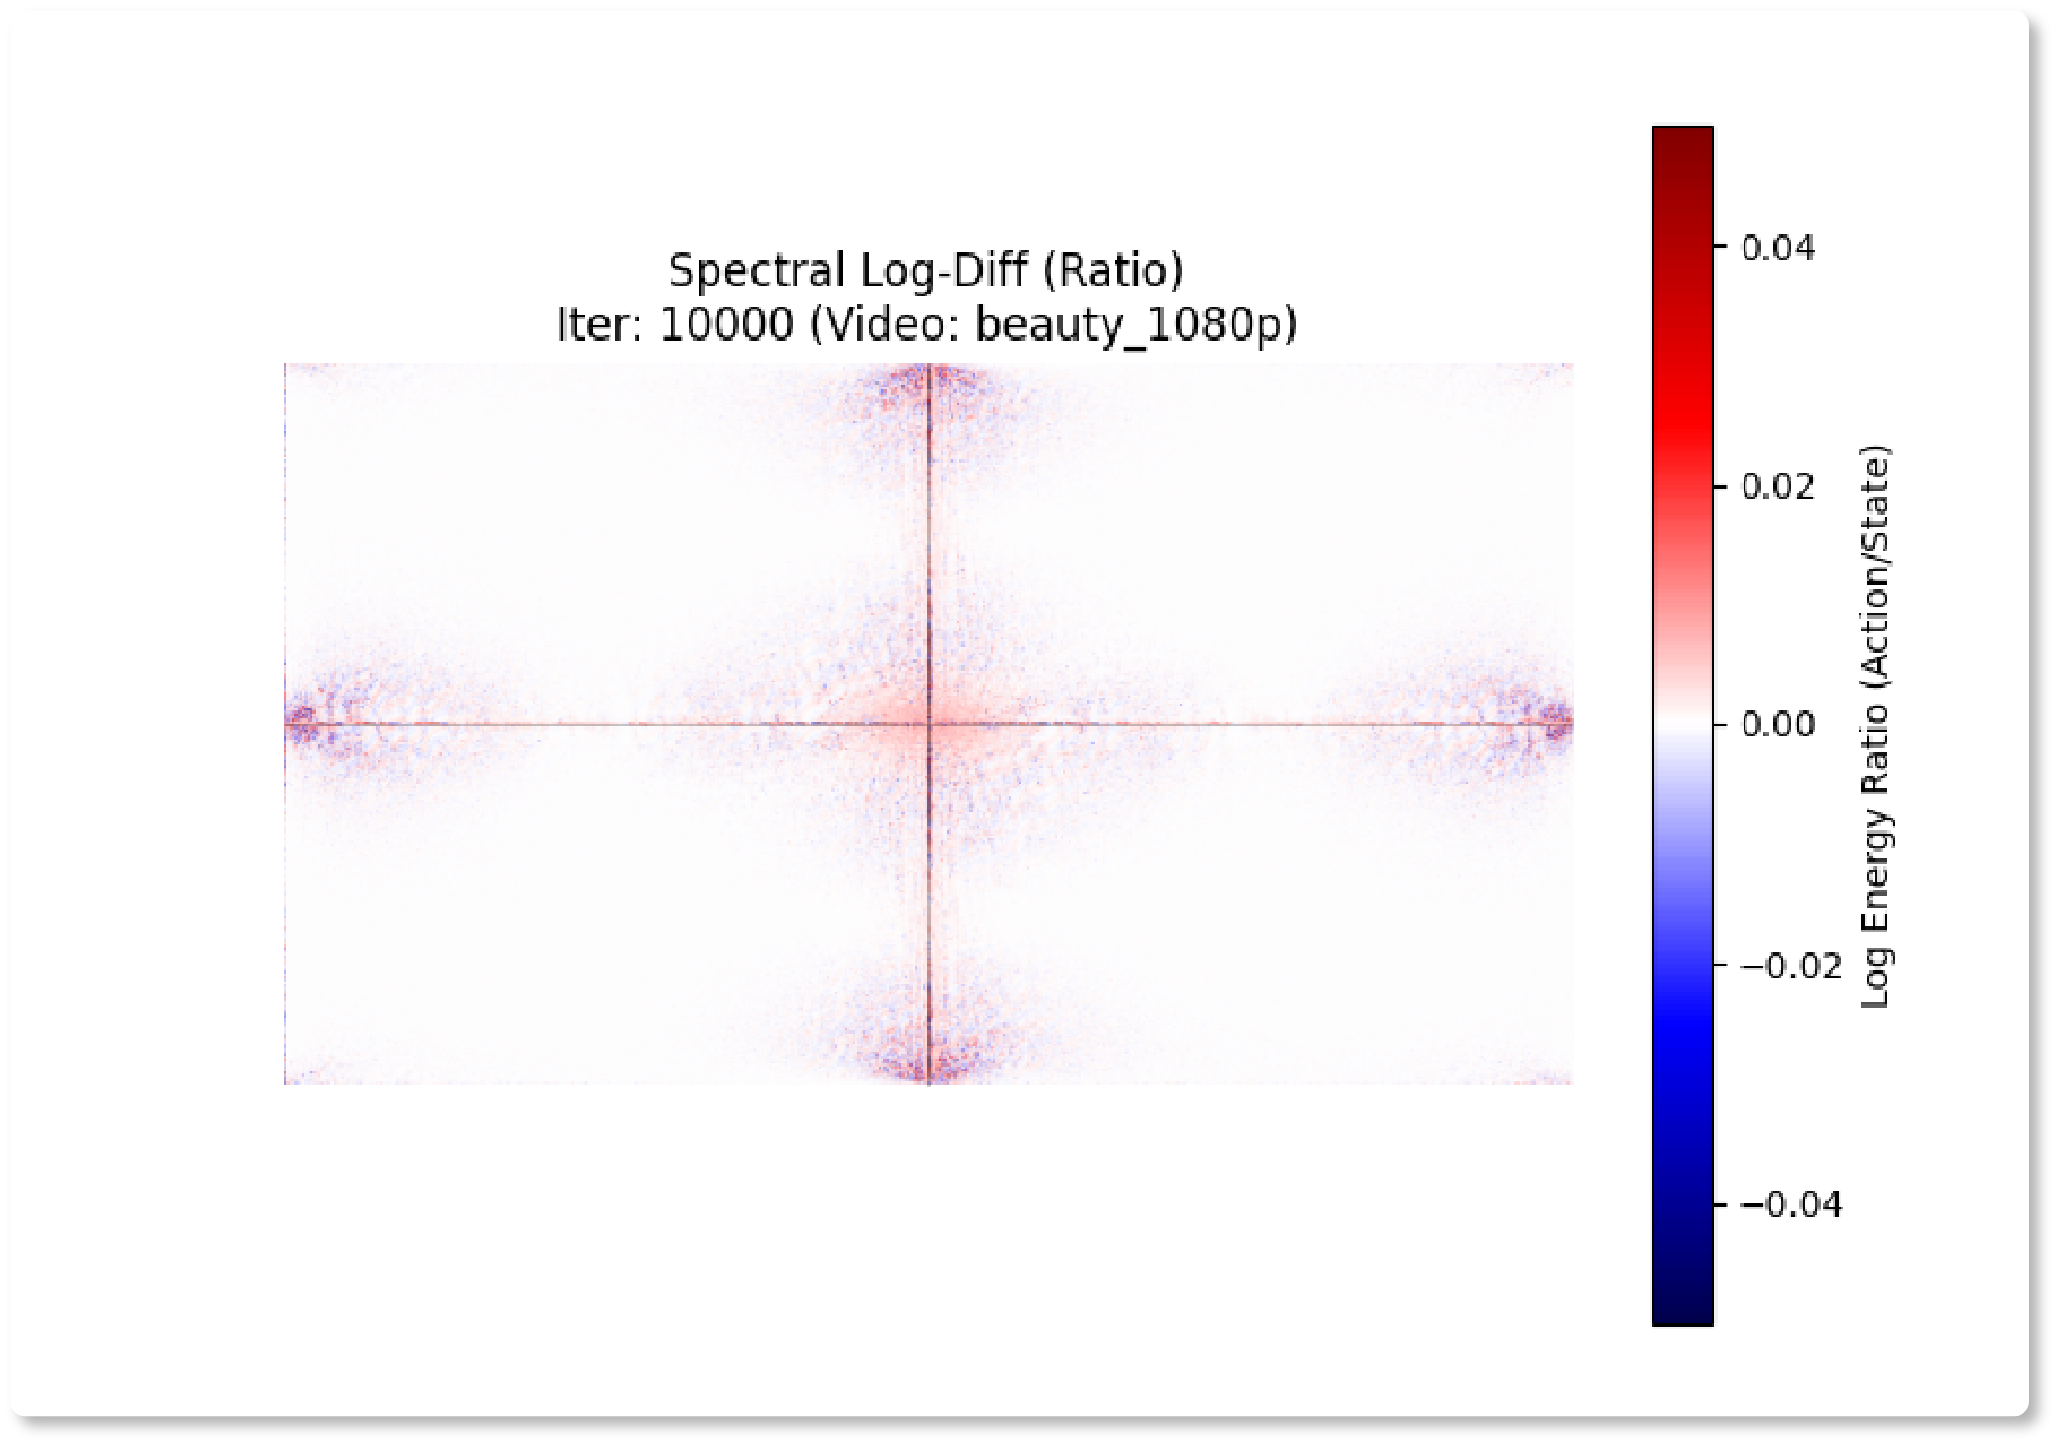
\includegraphics[width=0.75\textwidth]{data/图片模型处理后频谱图.png}
  \caption{模型处理前后频谱差异图（Spectral Log-Diff）}
  \label{fig:spectrum-analysis}
\end{figure}

\subsection{主观视觉效果分析}

% TODO: 插入主观质量对比图（Baseline vs RAPNet 的解码帧截图）


\section{消融实验}

为了验证系统设计中各关键参数的合理性，本节从编码参数选择和损失函数设计两个维度进行了系统性的消融实验。

\subsection{编码参数选择实验}

在正式训练强化学习模型之前，需要确定NVENC硬件编码器的最优参数配置。这些参数直接影响Baseline的率失真性能和训练环境的行为，因此需要通过迭代式实验来确定。

\subsubsection{NVENC Preset选择}

NVENC编码器提供p1至p7共7个编码预设，p1为最快速（最低质量），p7为最慢速（最高质量）。实验对p1至p4四个常用preset进行了编码质量与码率关系的对比分析，结果如图~\ref{fig:preset-compare}所示。

\begin{figure}[htbp]
  \centering
  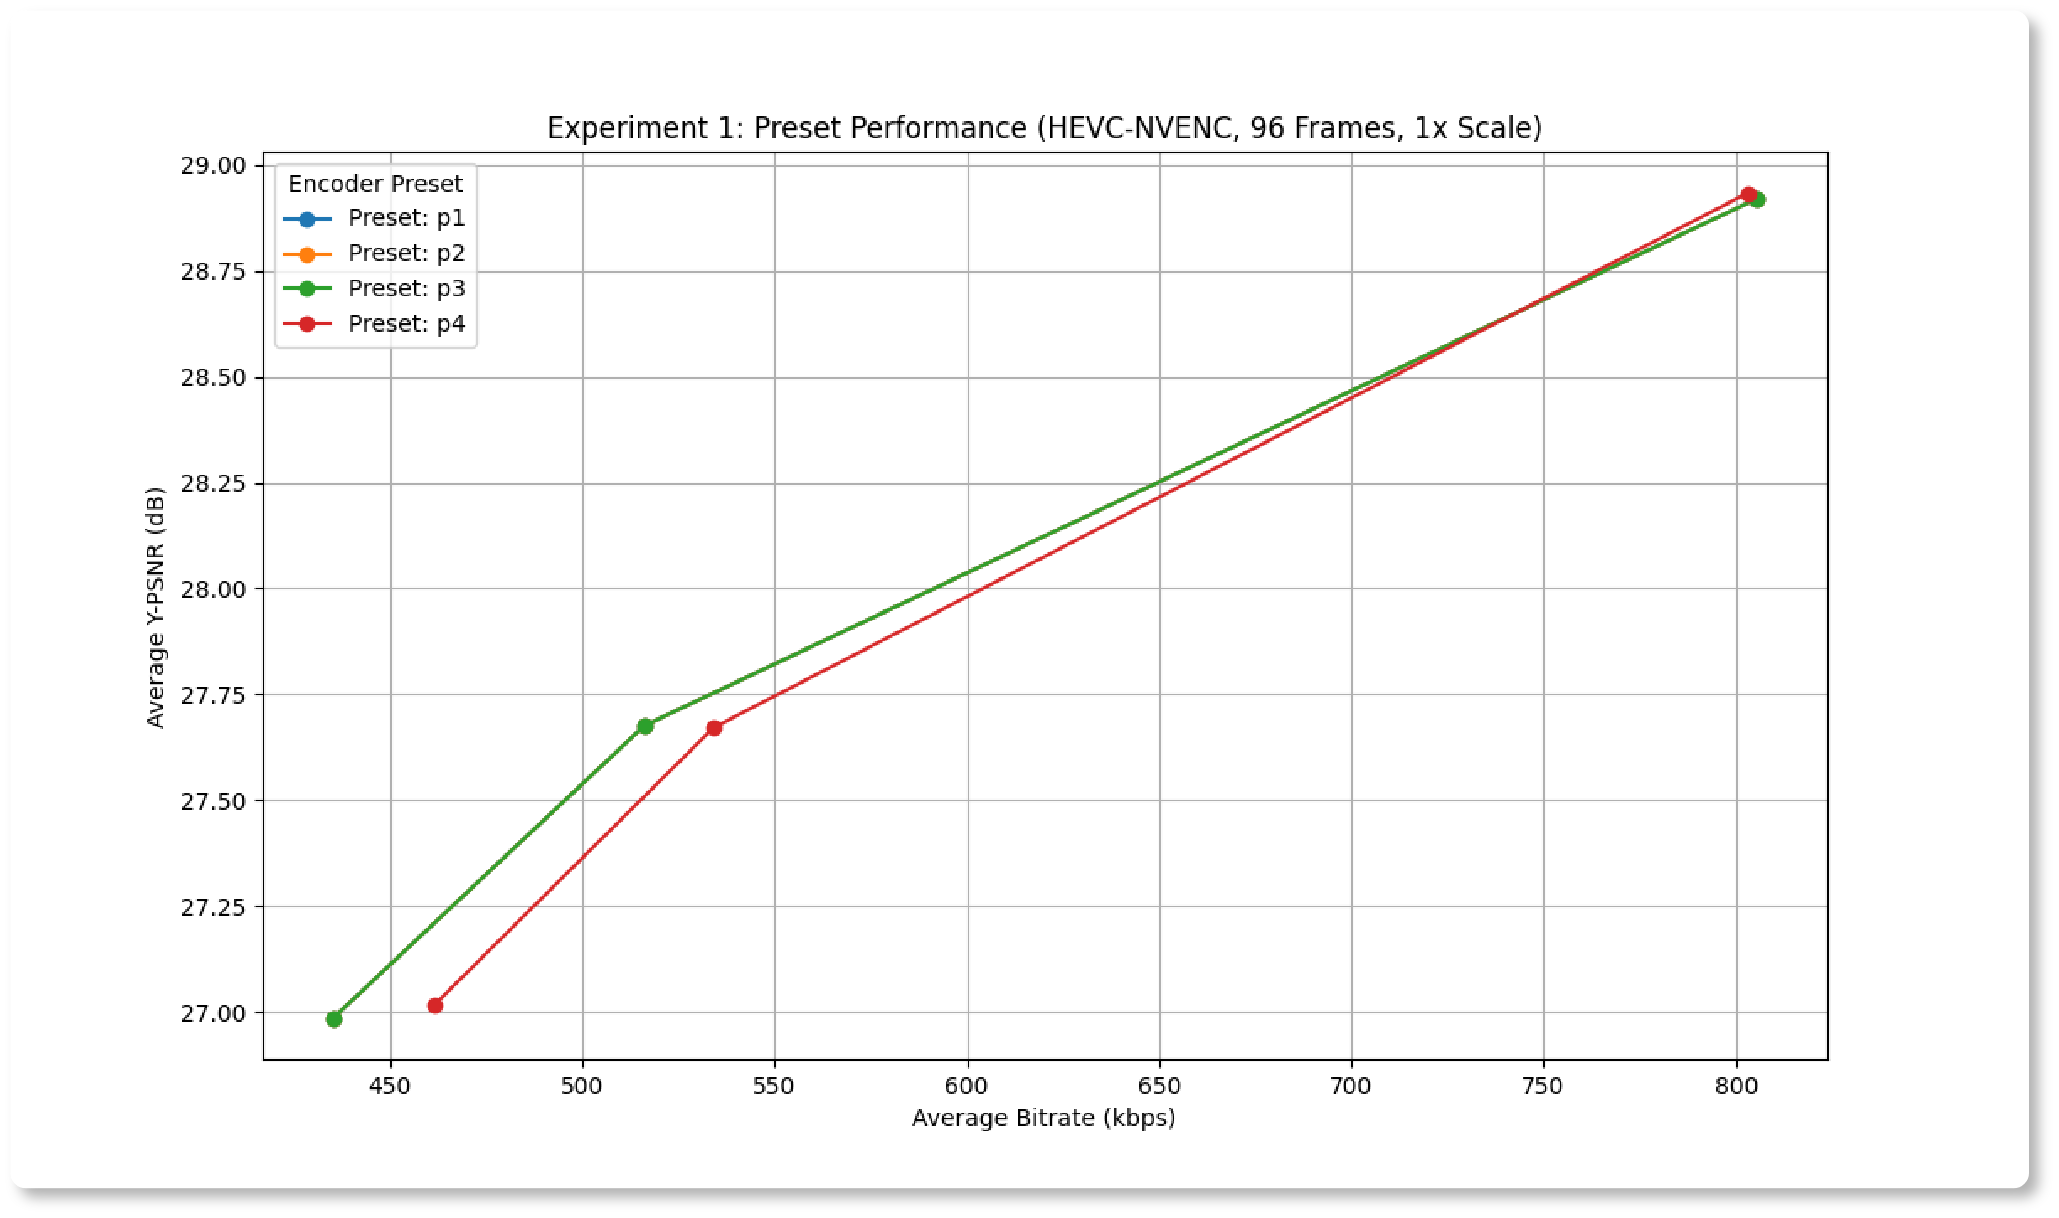
\includegraphics[width=0.8\textwidth]{data/图片Preset对比实验.png}
  \caption{NVENC编码预设对比实验（HEVC-NVENC, 96帧, 1x Scale）}
  \label{fig:preset-compare}
\end{figure}

从图~\ref{fig:preset-compare}可以看出，p1/p2/p3三个预设的RD曲线几乎完全重合，而p4在低码率点（400-600 kbps）上略低于p1-p3，但在高码率点上差异微乎其微。综合编码质量与训练速度，本文选择\textbf{p4 (medium)}作为训练和评估的统一预设。

GOP (Group of Pictures)定义了两个I帧之间的距离。在本文的训练场景中，每个episode编码16帧短clip，第一帧必须为I帧。图~\ref{fig:gop-compare}展示了GOP=$-1$（默认值）和GOP=32两种配置下，不同下采样算法的RD曲线对比。

\begin{figure}[htbp]
  \centering
  \begin{subfigure}[b]{0.48\textwidth}
    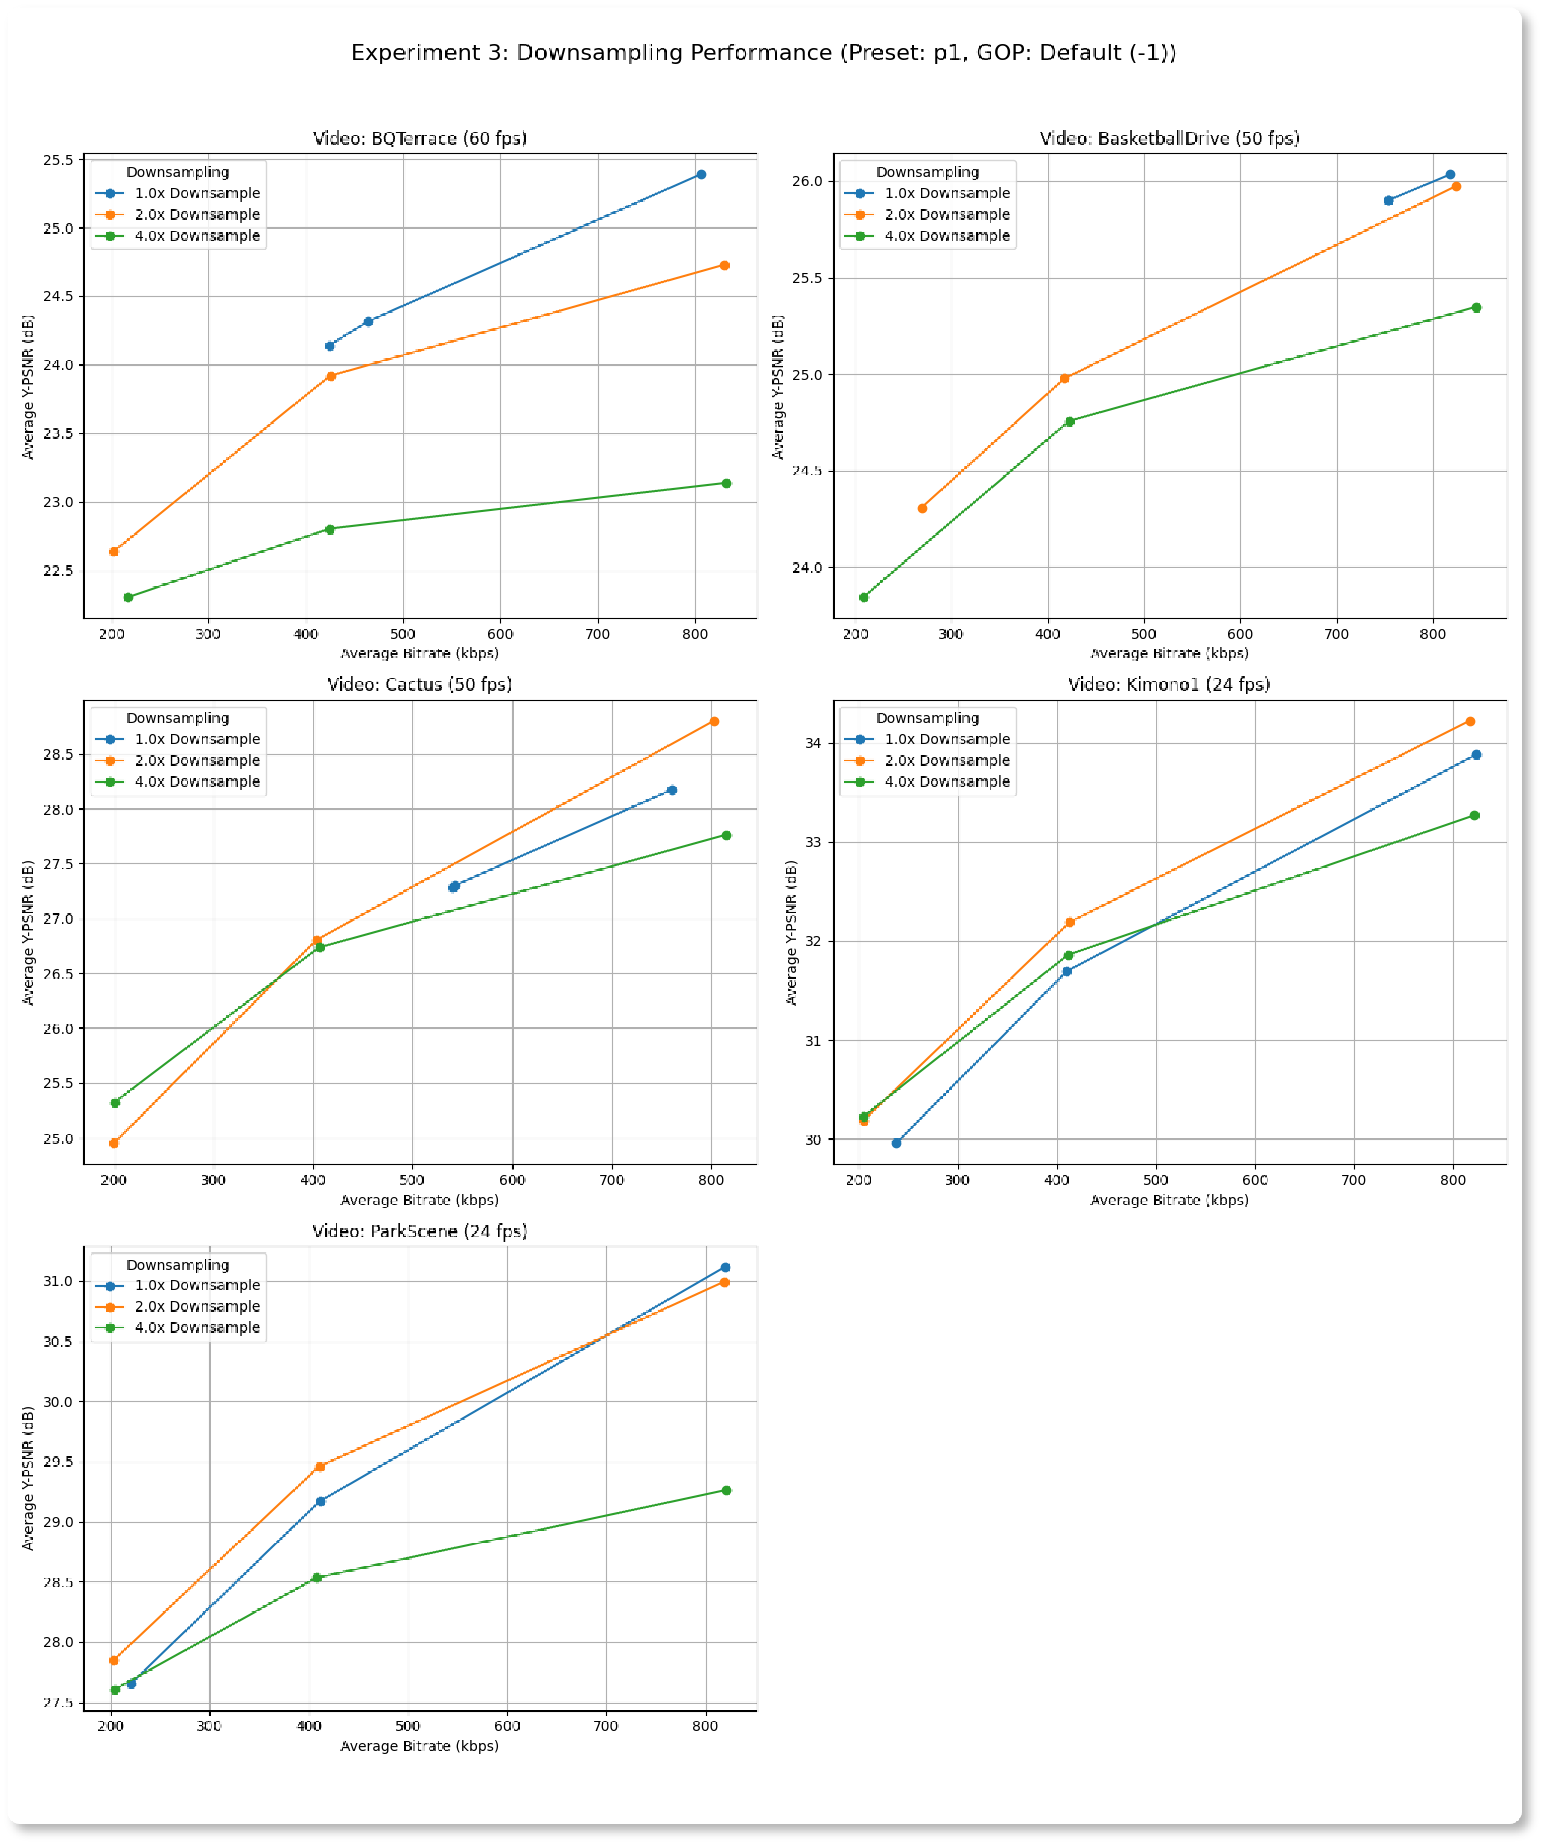
\includegraphics[width=\textwidth]{data/图片GOP = -1.png}
    \caption{GOP=$-1$（默认配置）}
    \label{fig:gop-default}
  \end{subfigure}
  \hfill
  \begin{subfigure}[b]{0.48\textwidth}
    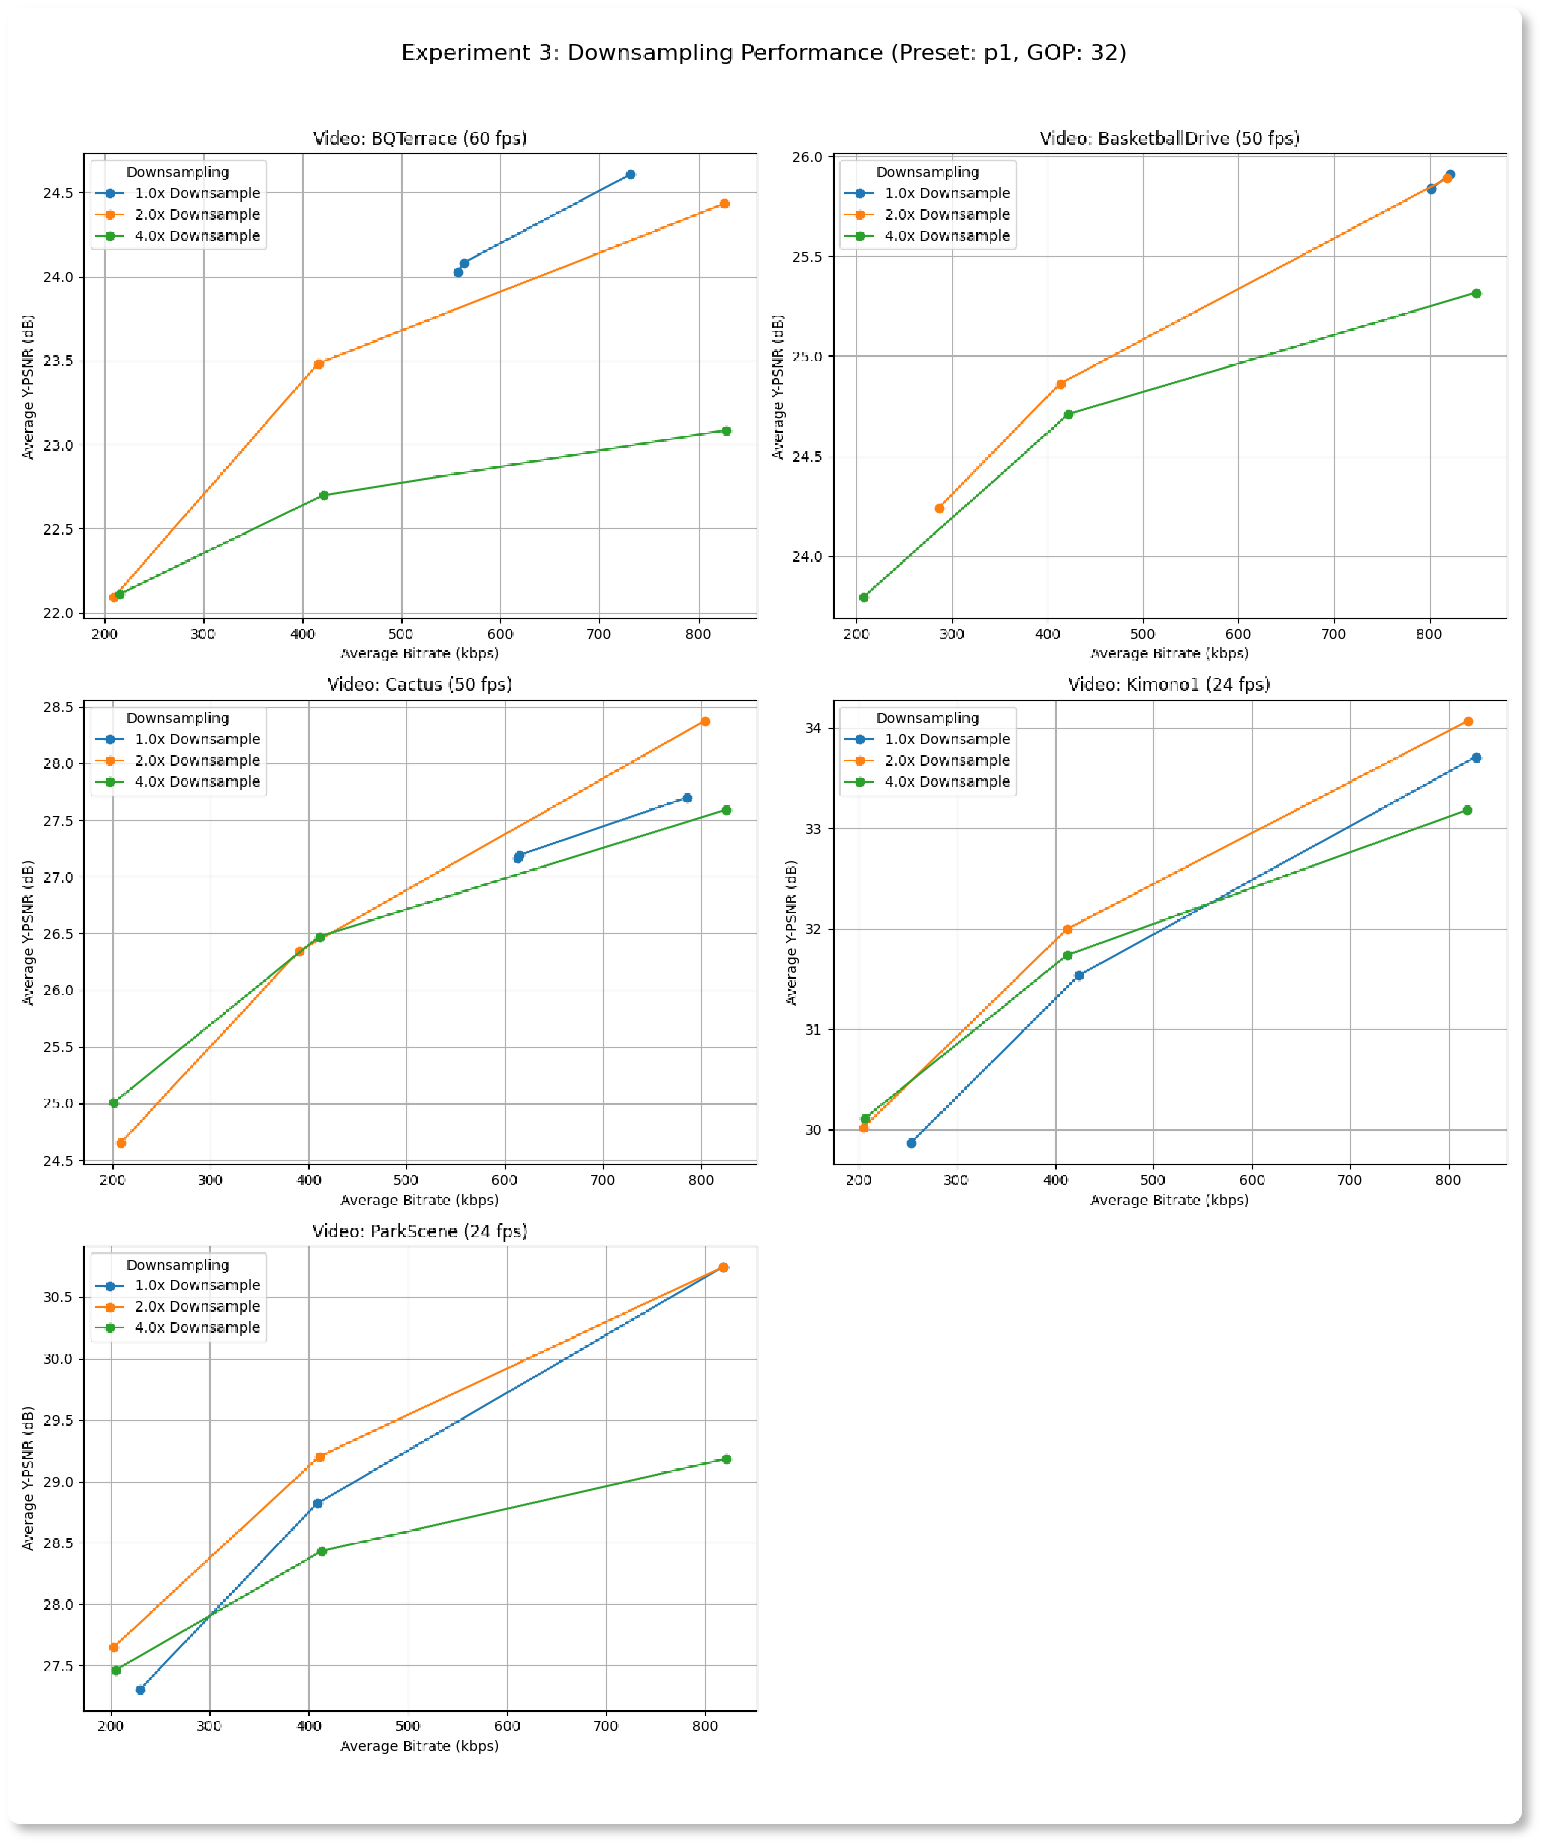
\includegraphics[width=\textwidth]{data/图片GOP=32.png}
    \caption{GOP=32}
    \label{fig:gop-32}
  \end{subfigure}
  \caption{不同GOP配置下的下采样算法RD曲线对比}
  \label{fig:gop-compare}
\end{figure}

从图~\ref{fig:gop-compare}可以观察到，GOP=32配置下各下采样算法的RD曲线整体低于GOP=$-1$配置，这是因为显式设置GOP=32会限制帧间预测的参考距离。经过实验验证，采用\textbf{GOP=$-1$（默认配置）}能够在训练稳定性和编码效率之间取得最佳平衡。

\subsubsection{色彩空间与像素格式}

视频编码标准普遍采用YCbCr色彩空间而非RGB，原因在于：（1）人眼对亮度（Y通道）的敏感度远高于色度（Cb/Cr通道），因此可以对色度进行4:2:0子采样而不显著影响主观质量；（2）Y/Cb/Cr三通道之间的相关性低于R/G/B通道，有利于后续的变换编码。

本系统全程在\textbf{YUV420p}格式下工作：亮度分辨率为$(H, W)$，色度分辨率为$(H/2, W/2)$。训练中需要特别注意：（1）PSNR等客观指标必须在YUV空间计算（Y-PSNR），而非在RGB空间计算，否则会导致结论偏差\footnote{FFmpeg在RGB输入时默认计算R/G/B PSNR，必须通过\texttt{format=yuv420p}强制转换为YUV后再计算。}；（2）随机裁剪坐标必须为2的倍数，以保证YUV420格式下亮度与色度通道的空间对齐。

\subsubsection{下采样算法选择}

在Baseline构建中，需要将1080p视频下采样到540p进行编码。不同的下采样算法对重建质量有显著影响。图~\ref{fig:downsample-compare}展示了5个测试序列在不同下采样倍数（1x/2x/4x）下的Y-PSNR对比。

\begin{figure}[htbp]
  \centering
  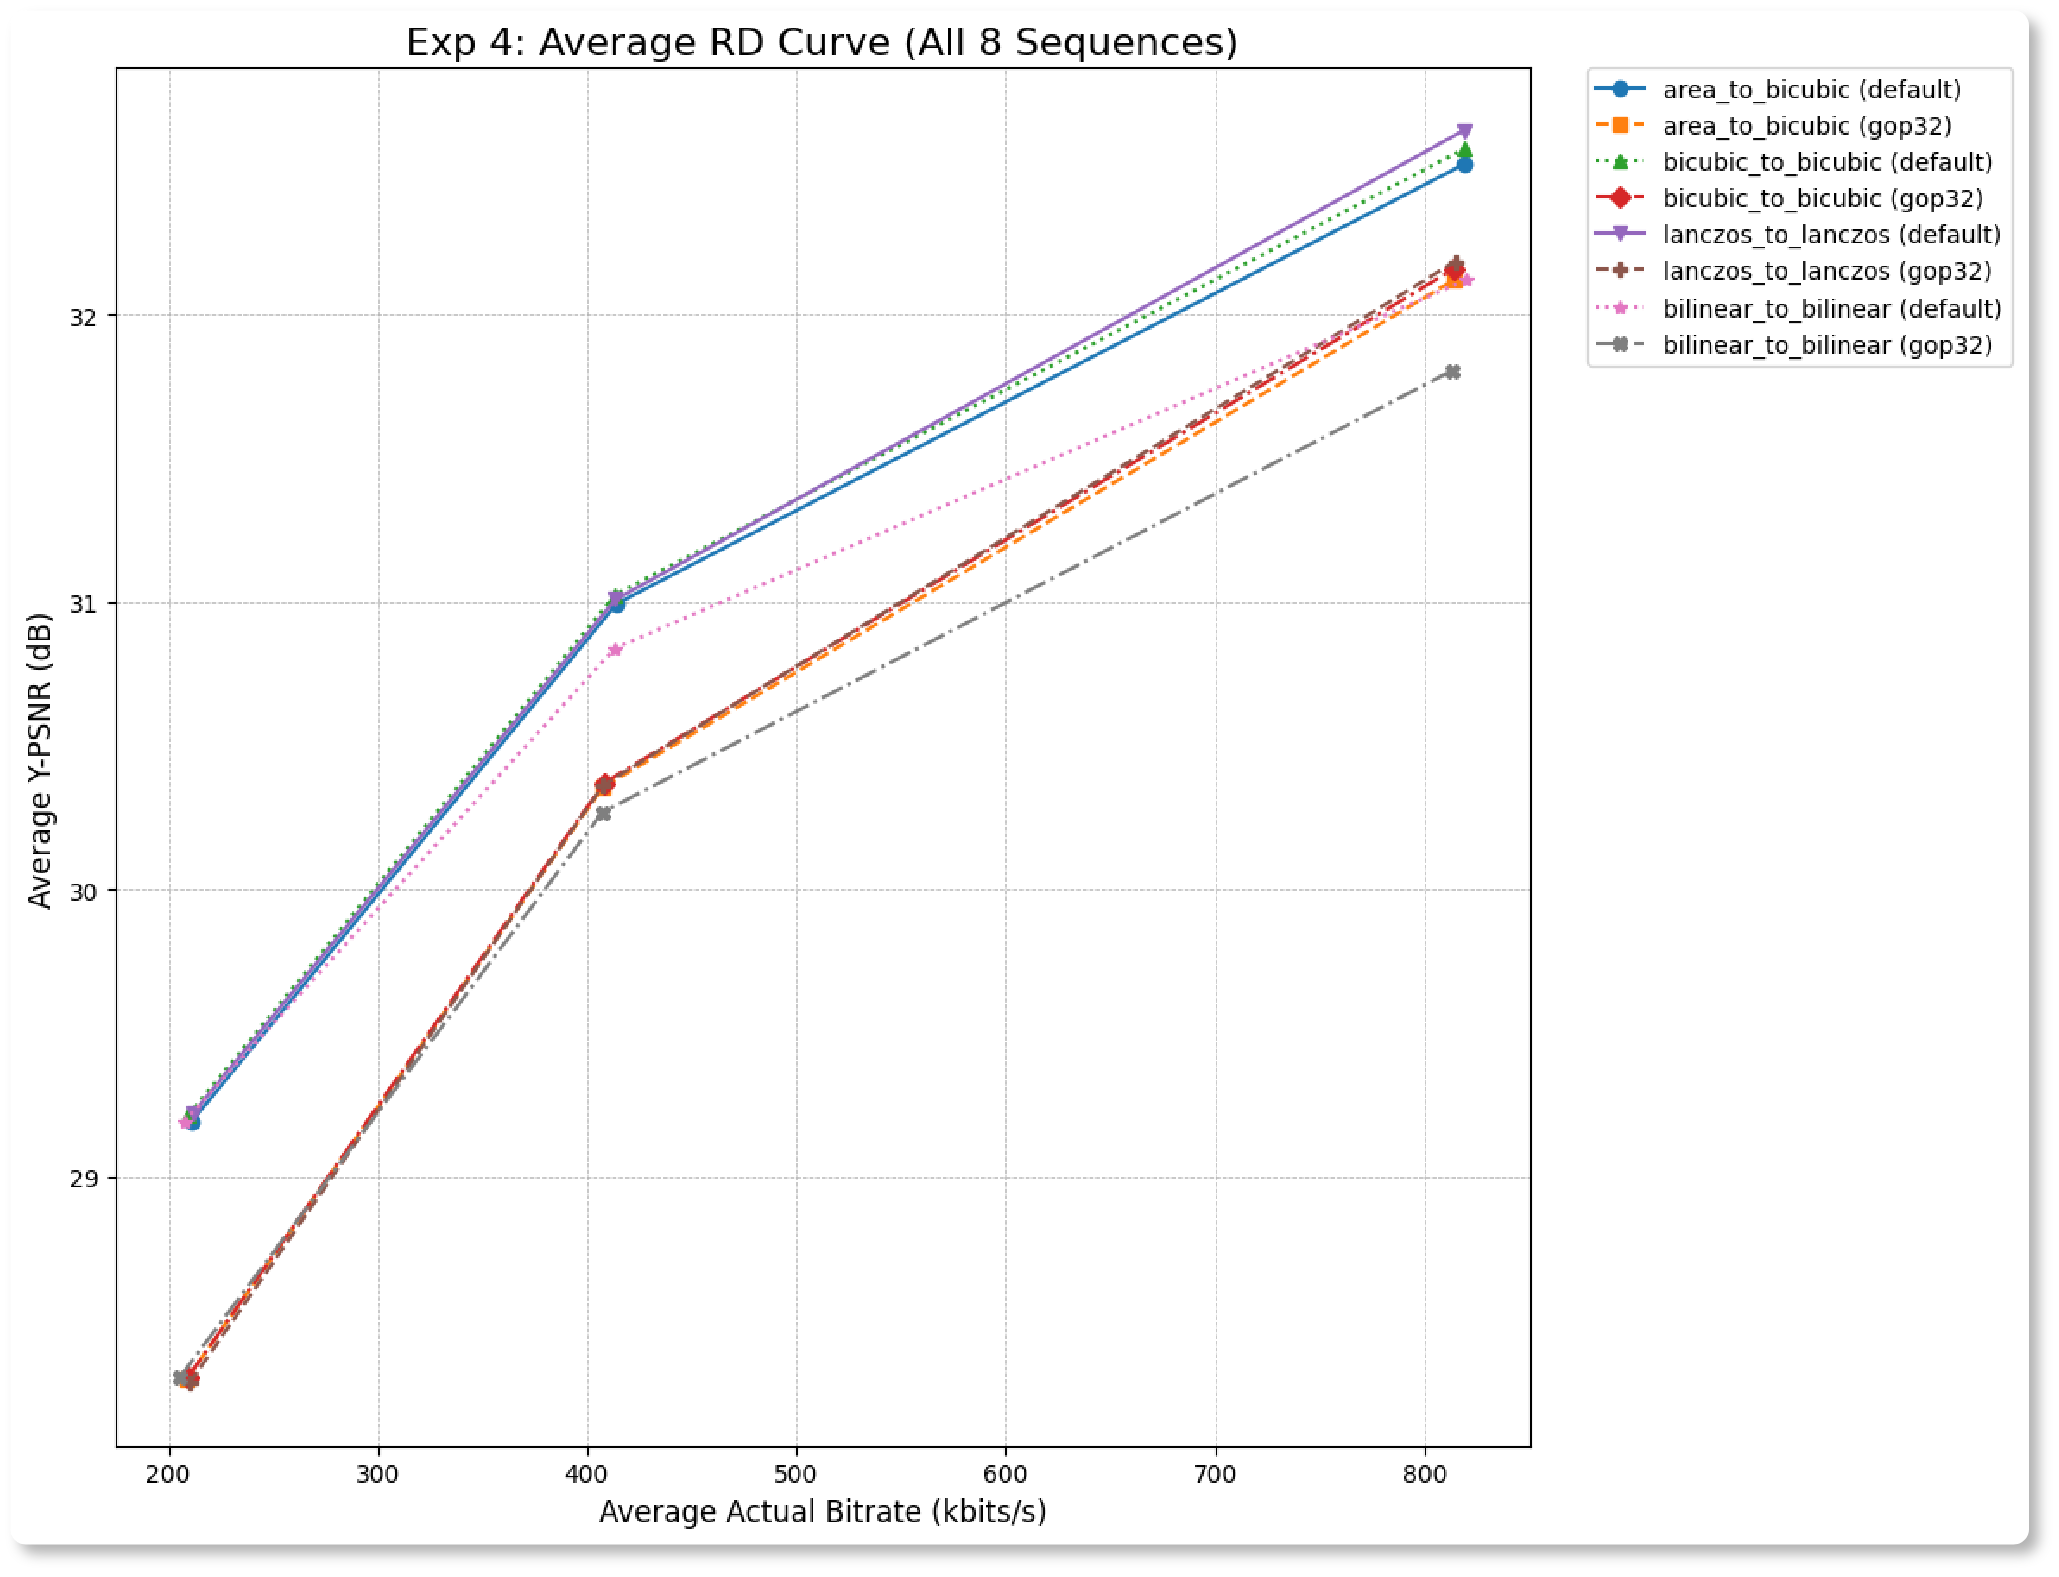
\includegraphics[width=0.85\textwidth]{data/图片下采样算法.png}
  \caption{不同下采样倍数下的Y-PSNR对比（Preset: p1, GOP: Default）}
  \label{fig:downsample-compare}
\end{figure}

从图~\ref{fig:downsample-compare}可以观察到：（1）1x（不下采样）始终提供最优的PSNR，但编码分辨率为原始1080p，码率开销最大；（2）2x下采样在中低码率点上表现良好，是本文采用的编码分辨率；（3）4x下采样导致PSNR显著下降，信息损失过大。结合图~\ref{fig:gop-compare}中的下采样算法对比，Lanczos算法在保持边缘锐度方面具有明显优势，因此本文在需要下采样的场景中统一采用Lanczos算法。

\subsubsection{码率控制模式}

NVENC支持多种码率控制模式，包括CQP（恒定QP）、CBR（恒定码率）和VBR（可变码率）等。本文选择\textbf{CQP (constqp)}模式，原因在于：（1）CQP模式下编码行为完全由QP值决定，消除了码率控制器引入的不确定性，使强化学习环境具有更好的可复现性；（2）CQP模式便于跨QP点的BD-Rate对比分析。

\subsection{损失函数消融实验}

为验证频域感知复合损失函数中各项的贡献，进行以下消融实验：

\begin{table}[htbp]
  \centering
  \caption{损失函数消融实验}
  \label{tab:ablation-loss}
  \begin{tabular}{lccc}
    \toprule
    \textbf{配置} & \textbf{BD-Rate(\%)} & \textbf{SSIM} & \textbf{LPIPS$\downarrow$} \\
    \midrule
    仅策略梯度损失 $-Q$                         & -- & -- & -- \\
    + MSE像素一致性 ($w_{mse}=0.3$)              & -- & -- & -- \\
    + 非边缘高频抑制 ($w_{hf}=0.5$)（完整方案）   & -- & -- & -- \\
    \bottomrule
  \end{tabular}
\end{table}

% TODO: 填入实际的消融实验数据

\subsection{训练策略消融}

为验证Random Crop训练策略的有效性，将其与传统的2$\times$下采样方案进行对比：

\begin{table}[htbp]
  \centering
  \caption{训练策略对比}
  \label{tab:ablation-crop}
  \begin{tabular}{lccc}
    \toprule
    \textbf{训练策略} & \textbf{BD-Rate(\%)} & \textbf{高频保持} & \textbf{边缘锐度} \\
    \midrule
    2$\times$下采样到540p   & -- & 差 & 差 \\
    Random Crop到540p     & -- & 好 & 好 \\
    \bottomrule
  \end{tabular}
\end{table}

% TODO: 填入实际对比数据

\subsection{模型参数量与推理速度}

\begin{table}[htbp]
  \centering
  \caption{模型效率对比}
  \label{tab:model-efficiency}
  \begin{tabular}{lccc}
    \toprule
    \textbf{模型} & \textbf{参数量} & \textbf{MACs(G)} & \textbf{单帧推理时间(ms)} \\
    \midrule
    RAPNet (Ours)\cite{ref27-zhao2025rapnet}  & $<$1M & -- & -- \\
    DnCNN\cite{ref5-ho2021rrdncnn}             & -- & -- & -- \\
    SwinIR\cite{ref25-liang2021swinir}         & -- & -- & -- \\
    VRT\cite{ref22-liang2022vrt}               & -- & -- & -- \\
    RVRT\cite{ref23-liang2022rvrt}             & -- & -- & -- \\
    BasicVSR++\cite{ref2-chan2021basicvsr}      & -- & -- & -- \\
    \bottomrule
  \end{tabular}
\end{table}

% TODO: 填入实际的模型效率数据


\section{本章小结}

本章首先搭建了包含硬件环境、软件环境和测试数据集的实验平台，定义了BD-LPIPS、LPIPS、PSNR等评价指标。在5个HEVC标准测试序列上的实验结果表明，RAPNet前处理框架取得了平均$-9.48\%$的BD-LPIPS增益，其中ParkScene和BasketballDrive序列分别达到$-13.45\%$和$-12.84\%$。频域分析显示，模型主要增强了水平和垂直方向的结构分量。在消融实验部分，系统性地验证了编码参数选择（preset、GOP、色彩空间、下采样算法、码率控制模式）的合理性，以及损失函数各项和Random Crop训练策略的贡献。

  % 第四章：实验与结果分析
\chapter{总结与展望}

\section{工作总结}

本文围绕实时约束下的可部署视频编码优化这一目标，研究了强化学习前处理与NVENC硬件编码器的协同机制。主要工作总结如下：

\begin{enumerate}
  \item 提出了一套包含前处理与后处理概念位的混合编码框架。本文重点对NVENC硬件编码前处理模块进行了实证验证，将不可导的闭源硬件编码器纳入优化回路，实现了前处理模型对编码器特性的感知与预补偿；

  \item 引入了基于Actor-Critic架构的RAPNet前处理网络，采用残差学习策略将动作空间约束为对原始帧的微调修正，并设计了基于相对率失真增益的复合奖励函数，使策略能够在质量与码率之间进行内容相关的自适应权衡；

  \item 提出了包含加权MSE损失、非边缘高频抑制损失和全变分平滑损失的频域感知复合损失策略，用于抑制增强过程中的高频伪影并提升输出稳定性；

  \item 在5个HEVC标准测试序列上，本文方法取得平均$-9.48\%$的BD-LPIPS收益，其中ParkScene和BasketballDrive分别达到$-13.45\%$与$-12.84\%$。在复杂度方面，模型参数量为139K、推理时延为5.4ms/帧，前处理开销约占端到端时延的12\%。这意味着在本文采用的NVENC实时编码链路中，额外引入5.4ms/帧前处理后，能够换取可测的感知率失真收益。
\end{enumerate}

\section{研究局限性与讨论}

在本文的研究与评测过程中，笔者也充分认识到了当前方案在理论与工程实践上的部分局限性，在此作补充讨论，以期为后续研究提供更严谨的视角：

\begin{enumerate}
  \item \textbf{强化学习与监督学习的权衡}：研究初期曾尝试更为直接的监督学习方案（如RPP），但后续研究转向强化学习。这一决策的根本原因在于应用场景，闭源NVENC硬件编码器不可导，且其码率控制算法对平滑信号极其敏感。监督学习缺乏来自真实编码器的环境反馈，容易出现客观指标较高但不适配硬件RC的情况。强化学习虽训练成本高、收敛更难，但在无梯度环境下通过实测反馈进行探索，在本文任务中更适合作为前处理与硬件编码器协同优化的方法。
  \item \textbf{客观评价指标的选取博弈}：本文在主要结果评测中着重汇报了LPIPS / BD-LPIPS，而非传统的PSNR。这是因为在低码率（200Kbps$\sim$800Kbps）的极端压缩工况下，重建画面通常伴随严重的块效应和振铃伪影。传统基于像素误差的PSNR往往对平滑但丧失纹理的画面给出高分，与人眼主观感知严重背离；而基于深度特征提取的LPIPS对结构失真和高频伪影有着更准确的惩罚机制，更能反映真实观感。
  \item \textbf{数据规模与外推的局限性}：当前系统仅使用5个UVG标准测试序列（1080p）进行了定量验证。虽然这类测试序列在课题研究中具有代表性，且覆盖了平坦、快速运动、复杂纹理等典型场景，但这毕竟属于中小规模评测。当前结论主要成立在针对HEVC编码、1080p分辨率与特定帧率的实时工程场景下。若要将结论外推至4K/8K超高清、非自然生成视频（如游戏录屏）或其他硬件平台，仍需更大规模的数据集与多样化编码器的进一步实验验证。
\end{enumerate}

\section{未来工作展望}

尽管本文已在既定实验条件下验证了方案的有效性，但受限于本科阶段可获取的计算资源、可覆盖的数据规模以及异构硬件平台条件，仍有若干更具系统性的工作尚未充分展开。后续研究可重点围绕以下三个方向推进：

\begin{enumerate}
  \item \textbf{更大规模与多分辨率的数据验证}：当前实验主要基于1080p标准测试序列展开，能够支持方法有效性的初步论证，但对更广泛内容分布的覆盖仍然有限。若要进一步扩展到2K、4K乃至更复杂场景，需要构建规模更大的训练与测试集，并完成大量离线编码与指标统计。这一过程对GPU算力、存储空间和实验周期都有较高要求，超出了当前毕业设计阶段的可承受范围，因此本文暂未进行更大规模的数据扩充与系统验证；

  \item \textbf{跨编码器与跨硬件平台的泛化评估}：本文工作主要围绕NVENC实时编码链路展开，结论目前仍建立在特定硬件平台与码率控制机制之上。若要将方法进一步推广到VVC、AV1或不同厂商的硬件编码器，除需重新适配实验链路外，还需要长期稳定获取多种GPU、移动端SoC或专用编解码设备。受当前平台条件限制，本文尚不具备完成大范围异构平台对比实验的硬件基础，后续可在条件允许时系统评估该方法的跨平台迁移能力；

  \item \textbf{面向真实系统的端到端部署研究}：离线实验已经表明前处理模块能够带来稳定的感知收益，但若要进入实际视频通信或流媒体系统，还需进一步考察端到端时延、显存占用、功耗波动与长期运行稳定性等工程指标。这类研究不仅需要完整的业务系统支撑，还依赖持续的联调、部署和性能剖析条件，而这些工作量已明显超出本文以算法验证为主的研究边界。后续若具备更完整的工程环境，可进一步开展真实业务场景下的部署验证与联合优化。
\end{enumerate}
  % 第五章：总结与展望

% ---- 参考文献 ----
\nocite{*}  % 暂时列出所有文献（正式提交时删除此行，只保留正文中 \cite 过的文献）
\printbibliography

% ---- 致谢 ----
\begin{acknowledgements}
  感谢导师黄公平教授在论文选题、研究过程及论文撰写中给予的悉心指导与帮助。感谢电子信息学院各位老师四年来的辛勤培养，感谢实验室同学们在实验调试和学术交流中的大力支持。感谢家人在求学路上始终如一的理解与鼓励。
  % ← 在此继续添加你的致谢内容
\end{acknowledgements}

% ---- 附录（如有代码清单等可在此添加）----
% \appendix
% % 附录
\chapter{关键实现说明}

由于完整工程代码体量较大，且包含训练脚本、模型定义、编码调用与评估工具等多个部分，为避免影响论文主体的连贯性，本文仅在附录中给出核心模块的详细结构、伪代码、主要参数配置及关键运行命令。完整代码作为毕业设计附件单独提交。

% ============================================================
\section{RAPNet (Actor) 详细网络结构}
% ============================================================

RAPNet采用``Pixel Unshuffle $\rightarrow$ 残差卷积 $\rightarrow$ Pixel Shuffle''的三段式架构，在低分辨率特征空间完成残差增强后映射回原分辨率。各层的具体参数如表~\ref{tab:rapnet-detail}所示。

\begin{table}[H]
  \centering
  \small
  \setlength{\tabcolsep}{4pt}
  \caption{RAPNet (Actor) 网络结构详情（$\text{scale}=2$时，$C_{in}=3 \times 2^2 = 12$）}
  \label{tab:rapnet-detail}
  \resizebox{\textwidth}{!}{%
  \begin{tabular}{llccl}
    \toprule
    \textbf{阶段} & \textbf{层名称} & \textbf{输入$\rightarrow$输出通道} & \textbf{核/步长/填充} & \textbf{激活} \\
    \midrule
    色度上采样 & \texttt{upsample\_chroma} & $(1,H/2,W/2)\rightarrow(1,H,W)$ & Bilinear $\times 2$ & — \\
    \midrule
    空间折叠 & \texttt{PixelUnshuffle(2)} & $(3,H,W)\rightarrow(12,H/2,W/2)$ & — & — \\
    \midrule
    主干入口 & \texttt{head} (Conv2d) & $12 \rightarrow 16$ & $3\times3$ / 1 / 1 & LeakyReLU(0.1) \\
    \midrule
    \multirow{2}{*}{残差体$\times 5$} & \texttt{body[i].conv1} & $16 \rightarrow 16$ & $3\times3$ / 1 / 1 & LeakyReLU(0.1) \\
     & \texttt{body[i].conv2} & $16 \rightarrow 16$ & $3\times3$ / 1 / 1 & 残差连接 \\
    \midrule
    主干出口 & \texttt{tail} (Conv2d) & $16 \rightarrow 12$ & $3\times3$ / 1 / 1 & — \\
    \midrule
    空间展开 & \texttt{PixelShuffle(2)} & $(12,H/2,W/2)\rightarrow(3,H,W)$ & — & — \\
    \midrule
    残差限幅 & $\delta = \tanh(\cdot) \times 0.05$ & — & — & Tanh \\
    色度均值归零 & $\delta_{Cb/Cr} \mathrel{-}= \text{mean}(\delta_{Cb/Cr})$ & — & — & — \\
    \midrule
    色度下采样 & \texttt{downsample\_chroma} & $(1,H,W)\rightarrow(1,H/2,W/2)$ & Bilinear $\times 0.5$ & — \\
    \bottomrule
  \end{tabular}
  }
\end{table}

总参数量约113K。其中5个ResBlock贡献了主要参数量（每个ResBlock含两层$16\rightarrow16$的Conv2d，参数$2\times(16\times16\times3\times3+16) = 4\,640$，五个共$23\,200$），head/tail的$12\leftrightarrow16$通道转换各贡献约$1\,744 / 1\,740$参数。

% ============================================================
\section{ValueNet (Critic) 详细网络结构}
% ============================================================

ValueNet采用双分支对称结构，分别对原始帧（状态$s$）和增强帧（动作$a$）提取特征，拼接后进行融合，最终输出标量Q值。各层的具体参数如表~\ref{tab:valuenet-detail}所示。

\begin{table}[!htbp]
  \centering
  \small
  \setlength{\tabcolsep}{4pt}
  \caption{ValueNet (Critic) 网络结构详情}
  \label{tab:valuenet-detail}
  \resizebox{\textwidth}{!}{%
  \begin{tabular}{llccl}
    \toprule
    \textbf{阶段} & \textbf{层名称} & \textbf{输入$\rightarrow$输出通道} & \textbf{核/步长/填充} & \textbf{激活} \\
    \midrule
    \multirow{2}{*}{输入分支} & \texttt{branch\_in.conv1} & $3 \rightarrow 32$ & $3\times3$ / 1 / 1 & LeakyReLU(0.1) \\
     & \texttt{branch\_in.conv2} & $32 \rightarrow 32$ & $3\times3$ / 1 / 1 & — \\
    \midrule
    \multirow{2}{*}{输出分支} & \texttt{branch\_out.conv1} & $3 \rightarrow 32$ & $3\times3$ / 1 / 1 & LeakyReLU(0.1) \\
     & \texttt{branch\_out.conv2} & $32 \rightarrow 32$ & $3\times3$ / 1 / 1 & — \\
    \midrule
    特征拼接 & \texttt{cat(in, out)} & $32+32=64$ & — & — \\
    融合卷积 & \texttt{fusion\_conv} & $64 \rightarrow 64$ & $3\times3$ / 1 / 1 & LeakyReLU(0.1) \\
    \midrule
    全局池化 & \texttt{AdaptiveAvgPool2d(1)} & $(64,H,W)\rightarrow(64,1,1)$ & — & — \\
    时间平均 & $\text{mean}(\cdot, \text{dim}=T)$ & $(B,T,64)\rightarrow(B,64)$ & — & — \\
    \midrule
    \multirow{2}{*}{MLP头} & \texttt{head.fc1} & $64 \rightarrow 64$ & — & ReLU \\
     & \texttt{head.fc2} & $64 \rightarrow 1$ & — & — \\
    \bottomrule
  \end{tabular}
  }
\end{table}

% ============================================================
\Needspace{0.7\textheight}
\section{损失权重与训练超参数}
% ============================================================

表~\ref{tab:hyperparams}汇总了模型在DDPG风格Actor-Critic训练框架中的完整超参数配置。这些参数来自最终收敛版本（v44），此前经历了近50个版本的迭代调参。

\begingroup
\small
\setlength{\tabcolsep}{4pt}
\setlength{\LTleft}{0pt plus 1fill}
\setlength{\LTright}{0pt plus 1fill}
\begin{longtable}{lll}
  \caption{训练主要超参数配置}
  \label{tab:hyperparams}\\
  \toprule
  \textbf{类别} & \textbf{超参数} & \textbf{设定值} \\
  \midrule
  \endfirsthead
  \caption[]{训练主要超参数配置（续）}\\
  \toprule
  \textbf{类别} & \textbf{超参数} & \textbf{设定值} \\
  \midrule
  \endhead
  \midrule
  \multicolumn{3}{r}{续下页} \\
  \endfoot
  \bottomrule
  \endlastfoot
  \multirow{4}{*}{迭代与数据}
    & 训练总迭代次数 & $20\,000$ \\
    & 每次采样帧数 (clip\_len) & 16 \\
    & 输入分辨率 & $1920 \times 1080$ \\
    & Random Crop裁剪尺寸 & $960 \times 540$ \\
  \midrule
  \multirow{4}{*}{学习率}
    & Actor学习率 $\eta_{Actor}$ & $1 \times 10^{-5}$ \\
    & Critic学习率 $\eta_{Critic}$ & $2 \times 10^{-5}$ \\
    & 学习率衰减步长 & 每1000 iter \\
    & 学习率衰减因子 $\gamma_{lr}$ & $1/3$ \\
  \midrule
  \multirow{3}{*}{奖励函数}
    & 质量权重 $\alpha$ & $200$ \\
    & 码率权重 $\beta$ & $100$ \\
    & QP测试点集 $\mathcal{Q}$ & $\{37, 40, 42, 45, 47\}$ \\
  \midrule
  \multirow{3}{*}{Actor损失权重}
    & MSE结构损失 $w_{mse}$ & $5$ \\
    & 非边缘高频抑制 $w_{hf}$ & $10$ \\
    & TV平滑损失 $w_{TV}$ & $0.1$ \\
  \midrule
  \multirow{2}{*}{残差限幅}
    & Tanh缩放系数 & $0.05$（即$\pm 5\%$） \\
    & Cb/Cr通道 & 零均值约束 \\
  \midrule
  \multirow{2}{*}{硬件分配}
    & Actor & GPU 0 (cuda:0) \\
    & Critic & GPU 1 (cuda:1) \\
\end{longtable}
\endgroup

\FloatBarrier

% ============================================================
\section{FFmpeg编码/解码命令示例}
% ============================================================

训练环路中的编码与解码通过Python \texttt{subprocess}调用FFmpeg完成。以下是从代码中提取的典型FFmpeg命令结构：

\noindent\textbf{编码命令}（NVENC HEVC硬件编码，恒定QP模式）：
\begin{lstlisting}[language=bash,basicstyle=\ttfamily\small,breaklines=true]
ffmpeg -y \
  -f rawvideo -pix_fmt yuv420p \
  -s:v 960x540 -r ${fps} \
  -i input_crop.yuv \
  -c:v hevc_nvenc \
  -rc constqp -qp 42 \
  -preset p4 -profile:v main \
  -pix_fmt yuv420p \
  output.hevc
\end{lstlisting}

\noindent\textbf{解码命令}（HEVC $\rightarrow$ 原始YUV420）：
\begin{lstlisting}[language=bash,basicstyle=\ttfamily\small,breaklines=true]
ffmpeg -y \
  -i output.hevc \
  -f rawvideo -pix_fmt yuv420p \
  decoded.yuv
\end{lstlisting}

\noindent 其中，\texttt{-rc constqp}表示恒定QP码率控制模式。训练阶段遍历5个QP点，即$\mathcal{Q}=\{37,40,42,45,47\}$，并对奖励取平均。\texttt{-preset p4}对应NVENC的Medium编码预设，\texttt{-r \${fps}}表示按当前序列原始帧率设置时间基准，例如BasketballDrive/Cactus为50fps，ParkScene/Kimono1为24fps，BQTerrace为60fps。

% ============================================================
\section{核心代码文件目录说明}
% ============================================================

随论文提交的代码附件已整理为\texttt{毕业论文代码/}目录。该目录只包含论文复现实验所需的源码、工具脚本、依赖说明与模型权重；标准YUV测试序列体积较大，需按本地环境另行放置并修改脚本中的数据集路径。主要文件组织结构如下：

\begin{lstlisting}[basicstyle=\ttfamily\small]
毕业论文代码/
+-- README.md
+-- requirements.txt
+-- src/
|   +-- rapnet_hevc_ppo_qp_yuv_1080p.py
|   |     # 最终1080p Random Crop训练脚本
|   |     # 包含: RAPNetYCbCr (Actor),
|   |     #       ValueNetYCbCrPair (Critic),
|   |     #       DeterministicACAgentYCbCr,
|   |     #       NvencClipEnvQP,
|   |     #       train_rapnet_with_config()
|   +-- rapnet_hevc_ppo_qp_yuv_simple.py
|   |     # 下采样版本训练与完整视频评估依赖脚本
|   +-- gradient_monitor.py
|         # Actor-Critic梯度诊断工具
+-- tools/
|   +-- eval_rapnet_full_video.py
|   |     # 完整视频推理与RD评估脚本
|   +-- evaluate_time.py
|   |     # 读入、前处理、编码、解码端到端耗时统计
|   +-- run_ablation_3variants.py
|         # 三组损失配置消融实验自动化脚本
+-- checkpoints/
|   +-- actor_best.pth
|   +-- critic_best.pth
+-- results/
|     # 放置Baseline RD曲线JSON与评估输出
+-- tmp/
      # FFmpeg编码/解码临时文件目录
\end{lstlisting}

\FloatBarrier

% ============================================================
\chapter{代码提交说明}
% ============================================================

本课题完整代码已随毕业设计材料以\texttt{毕业论文代码/}目录形式提交。代码附件主要包括以下文件：

\begin{itemize}
  \item \path{src/rapnet_hevc_ppo_qp_yuv_1080p.py}：最终采用的1080p Random Crop训练入口；
  \item \path{src/rapnet_hevc_ppo_qp_yuv_simple.py}：下采样版本训练与完整视频评估所需的公共函数；
  \item \path{tools/eval_rapnet_full_video.py}：完整视频推理与RD评估脚本；
  \item \path{tools/evaluate_time.py}：端到端耗时统计脚本；
  \item \path{tools/run_ablation_3variants.py}：三组损失配置消融实验脚本；
  \item \path{checkpoints/actor_best.pth}与\path{checkpoints/critic_best.pth}：最终提交的最优Actor与Critic权重。
\end{itemize}

为避免论文附录过长，本文不在附录中逐行粘贴完整Python源码，而是给出关键网络结构、训练参数、编码命令和文件组织说明。复现实验时，可先根据\path{requirements.txt}安装依赖，再准备HEVC CTC Class B和UVG等YUV420测试序列，并将脚本中的\texttt{VIDEO\_META\_LIST}路径改为本机数据集路径。Baseline RD曲线JSON可由训练脚本中的Baseline构建函数生成，也可放置于\path{results/}目录后通过环境变量\texttt{RAPNET\_BASELINE\_JSON}指定。

如需复现实验结果，请确保以下环境配置：
\begin{itemize}
  \item NVIDIA GPU $\times$ 2（推荐RTX 4090或同等级别，显存$\geq$16GB）
  \item CUDA 12.x + cuDNN 9.x
  \item Python 3.10+, PyTorch 2.0+
  \item FFmpeg 6.0+（需包含\texttt{hevc\_nvenc}编码器支持）
  \item 关键Python包：\texttt{lpips}, \texttt{tensorboard}, \texttt{numpy}, \texttt{opencv-python}
\end{itemize}


\end{document}
